\section{The compressible Navier-Stokes equations}

We briefly review the 2D compressible Navier-Stokes equations and formulate DPG for the nonlinear system. 
\begin{itemize}
\item \textbf{Conservation equations}
\begin{align*}
\div \vecttwo{\rho u_1 }{\rho u_2} &= 0\\
\div \vecttwo{\rho u_1^2+p }{\rho u_1 u_2} &= \div\left(\vec{\sigma_{i1}}\right)\\
\div \vecttwo{\rho u_1 u_2}{\rho u_2^2+p } &= \div\left(\vec{\sigma_{i2}}\right)\\
\div\vecttwo{((\rho e)+p)u_1}{((\rho e)+p)u_2} &= \div\left[\boldsymbol\sigma \boldsymbol u + \vec{q}\right],
\end{align*}
where $\boldsymbol \sigma$ is the stress tensor whose $ij$th term is $\sigma_{ij}$, and $\boldsymbol u$ is the vector $(u_1,u_2)^T$.  

\item \textbf{Newtonian fluid laws}

We represent $\boldsymbol\sigma$ using the Newtonian fluid law
\[
\sigma_{ij} = \mu(u_{i,j} + u_{j,i}) + \lambda u_{k,k} \delta_{ij}
\]
where $\mu$ is viscosity and $\lambda$ is bulk viscosity. 
%Following elasticity, a general formula for the stress tensor is 
%\[
%\sigma_{ij} = 2\mu \epsilon_{ij} + \lambda \epsilon_{kk} \delta_{ij}
%\]
We can invert the stress tensor under isotropic and plane strain assumptions to get
\[
\frac{1}{2}\left(\grad  \boldsymbol u + \grad ^T  \boldsymbol u\right) = \frac{1}{2\mu} \sigma_{ij} - \frac{\lambda}{4\mu (\mu + \lambda)} \sigma_{kk}\delta_{ij}
\]
We also have
\[
\frac{1}{2}\left(\grad  \boldsymbol u + \grad ^T  \boldsymbol u\right) = \grad  \boldsymbol u - \boldsymbol \omega
\]
where $\boldsymbol \omega$ is the antisymmetric part of the infinitesimal strain tensor:
\[
\boldsymbol \omega = \frac{1}{2}\left(\grad  \boldsymbol u - \grad ^T  \boldsymbol u\right).
\]
Thus our final form is
\begin{align*}
\grad  \boldsymbol u - \boldsymbol \omega = \frac{1}{2\mu} \boldsymbol \sigma - \frac{\lambda}{4\mu (\mu + \lambda)} { \rm tr}(\boldsymbol \sigma) \boldsymbol I.
\end{align*}
Notice that $\boldsymbol \omega$ is implicitly defined to be the antisymmetric part of $\grad u$ by taking the symmetric part of the above equation. 

We note that, though this is a standard approach in solid mechanics, it is nonstandard compared to the usual finite element and DG approaches to the viscous stresses. We adopt such an approach to better mirror our experiences with the convection-diffusion equation \cite{DPGrobustness,DPGrobustness2}. 

\item \textbf{Fourier's heat conduction law}

We assume Fourier's law 
\begin{align*}
\vec{q} &= \kappa \grad T,
\end{align*}
%where $\kappa$ is generally a function of temperature. 
We introduce here the Prandtl number here as well
\[
{\rm Pr} = \frac{\gamma c_v \mu}{\kappa}.
\]
In this case, we assume a constant Prandlt number, which implies that the heat conductivity $\kappa$ is proportional to viscosity $\mu$.

\end{itemize}

\subsection{Nondimensionalization}
To nondimensionalize our equations, we introduce nondimensional quantities for length, density, velocity, temperature, and viscosity. 
\[
\boldsymbol x^* = \frac{\boldsymbol x}{L}, \qquad \rho^* = \frac{\rho}{\rho_{\infty}}, \qquad u_1^* = \frac{u_1}{V_\infty}, \qquad u_2^* = \frac{u_2}{V_\infty}, \qquad T^* = \frac{T}{T_\infty}, \qquad \mu^* = \frac{\mu}{\mu_\infty}
\]
Pressure, internal energy, and bulk viscosity are then nondimensionalized with respect to the above variables
\[
p^* = \frac{p}{\rho_\infty V_\infty^2}, \qquad \iota^* = \frac{\iota}{V_\infty^2}, \qquad \lambda^* = \frac{\lambda}{\mu_\infty}
\]
We introduce, for convenience, the Reynolds number
\[
\Reyn = \frac{\rho_\infty V_\infty L}{\mu_\infty} 
\]
and the reference (free stream) Mach number
\[
M_\infty = \frac{V_\infty}{\sqrt{\gamma(\gamma-1)c_vT_\infty}}
\]
Note that 
\[
a = \sqrt{\frac{\gamma p_\infty}{\rho_\infty}} = \sqrt{{\gamma p_\infty}} = \sqrt{\gamma(\gamma-1)c_vT_\infty}
\]
The equations take the same form as before after nondimensionalization, so long as we define new material constants
\[
\tilde{\mu} = \frac{\mu^*}{\Reyn}, \qquad \tilde{\lambda} = \frac{\lambda^*}{\Reyn}, \qquad \tilde{c}_v = \frac{1}{\gamma(\gamma-1)M_\infty^2}, \qquad \tilde{\kappa} = \frac{\gamma\tilde{c}_v\tilde{\mu}}{\rm Pr}
\]
From here on, we drop the $^*$ superscript and assume all variables refer to their nondimensionalized quantities.

To summarize, our system of equations in the classical variables is now
\begin{align*}
\div \vecttwo{\rho u_1 }{\rho u_2} &= 0\\
\div \left(\vecttwo{\rho u_1^2+p }{\rho u_1 u_2} - \boldsymbol \sigma_{1}\right) &=0\\
\div \left(\vecttwo{\rho u_1 u_2}{\rho u_2^2+p } - \boldsymbol \sigma_{2}\right) &=0\\
\div \left(\vecttwo{((\rho e)+p)u_1}{((\rho e)+p)u_2} - \boldsymbol\sigma \mathbf{u} - \vec{q}\right) &=0\\
\frac{1}{2\mu} \boldsymbol \sigma - \frac{\lambda}{4\mu (\mu + \lambda)} { \rm tr}(\boldsymbol \sigma) \boldsymbol I &= \grad \mathbf{u} - \Reyn \, {\boldsymbol \omega}\\
\frac{1}{\kappa}\vec{q} &= \grad T
\end{align*}
We strongly enforce symmetry of the stress tensor $\boldsymbol \sigma$ by setting $\sigma_{21} = \sigma_{12}$. Additionally, we have scaled the antisymmetric tensor $\boldsymbol \omega$ by the Reynolds number to ensure that $\boldsymbol \omega = O(1)$ for all ranges of $\Reyn$.  

\subsection{Linearization}

As the equations for viscous compressible flow are nonlinear and cannot be solved exactly, we linearize the equations and adopt an iterative procedure for approximating the nonlinear solution.\footnote{We note that it is possible to linearize the strong form of the equations and then derive a linearized weak form, instead of linearizing the weak form of the nonlinear equations, which is done here.  The two formulations are equivalent; however, extraneous linearization of the fluxes is avoided using the latter approach.}  We outline the linearization of both the conservation and stress laws in this section.

\subsubsection{Conservation laws}

The Navier-Stokes conservation laws can be written as 
\begin{align*}
\div \vecttwo{\rho u_1 }{\rho u_2} &= 0\\
\div \left(\vecttwo{\rho u_1^2+p }{\rho u_1 u_2} - \boldsymbol \sigma_{1}\right) &=0\\
\div \left(\vecttwo{\rho u_1 u_2}{\rho u_2^2+p } - \boldsymbol \sigma_{2}\right) &=0\\
\div \left(\vecttwo{((\rho e)+p)u_1}{((\rho e)+p)u_2} - \boldsymbol \sigma_1 \cdot \boldsymbol u- \boldsymbol \sigma_2 \cdot \boldsymbol u - \vec{q}\right) &=0,
\end{align*}
where $\boldsymbol \sigma_1$ is the $i$th column or row of $\boldsymbol \sigma$, or more generally, if we group our Eulerian and stress variables into the vector variables $\boldsymbol U$ and $\boldsymbol \Sigma$, respectively
\[
\div (F_i(\boldsymbol U)-G_i(\boldsymbol U,\boldsymbol \Sigma) = 0, \qquad i = 1,\ldots, 4,
\]
where $F_i$and $G_i$ are given as
\begin{align*}
F_1 = \vecttwo{\rho u_1 }{\rho u_2}, \quad &G_1 = 0\\
F_2 = \vecttwo{\rho u_1^2+p }{\rho u_1 u_2},\quad &G_2 = \boldsymbol \sigma_{1}\\
F_3 = \vecttwo{\rho u_1 u_2}{\rho u_2^2+p }, \quad &G_3 = \boldsymbol \sigma_{2}\\
F_4 = \vecttwo{((\rho e)+p)u_1}{((\rho e)+p)u_2}, \quad &G_4 = \boldsymbol \sigma_1 \cdot \boldsymbol u + \boldsymbol \sigma_2 \cdot \boldsymbol u + \vec{q}
\end{align*}
The variational form restricted to a single element gives
\[
\langle \widehat{F}_i\cdot n, v\rangle - \int_K  (F(\boldsymbol U)-G_i(\boldsymbol U,\boldsymbol \Sigma)) \cdot \grad v_i = 0 , \qquad i = 1,\ldots, 4
\]
and the variational form over the entire domain is given by summing up the element-wise contributions. 

The presence of terms such as $\boldsymbol \sigma_i \cdot \boldsymbol u$ means that we will need to linearize in the stress variables $\sigma_ij$ in addition to our Eulerian quantities. Since fluxes and traces are linear functions of the unknowns, we do not need to linearize them. Instead, fluxes $\widehat{F}_{i,n}$ and traces $\widehat{u},\widehat{v},\widehat{T}$ will represent normal traces and traces of the accumulated nonlinear solution. The linearized variational formulation is thus
\begin{align*}
\langle \widehat{F}_i\cdot n, v\rangle &- \int_K  \left(F_{i,\boldsymbol U}(\boldsymbol U)\cdot \Delta \boldsymbol U -G_{i,\boldsymbol U}(\boldsymbol U, \boldsymbol \Sigma)\cdot \Delta \boldsymbol U - G_{i,\boldsymbol \Sigma}(\boldsymbol U, \boldsymbol \Sigma)\cdot \Delta \boldsymbol \Sigma \right)\cdot \grad v_i \\
&= \int_K  \left(F_i(\boldsymbol U)-G_i(\boldsymbol U)\right) \cdot \grad v_i \\
\qquad i &= 1,\ldots, 4
\end{align*}
where $F^i_{j,\boldsymbol U}$, $G^i_{j,\boldsymbol U}$, and $G^i_{j,\boldsymbol \Sigma}$ are the Eulerian and two viscous Jacobians (linearized w.r.t.\ the Eulerian/viscous variables), respectively.
%where
%\begin{align*}
%F^1_{1,\boldsymbol U} &= \{u,\rho ,0,0\} \\
%F^2_{1,\boldsymbol U} &= \{v,0,\rho ,0\} \\
%F^1_{2,\boldsymbol U} &=\left\{c_v T (\gamma -1)+u^2,2 u \rho ,0,c_v (\gamma -1) \rho \right\}\\
%F^2_{2,\boldsymbol U} &=\{u v,v \rho ,u \rho ,0\}\\
%F^1_{3,\boldsymbol U} &=\{u v,v \rho ,u \rho ,0\}\\
%F^2_{3,\boldsymbol U} &=\left\{c_v T (\gamma -1)+v^2,0,2 v \rho ,c_v (\gamma -1) \rho \right\}\\
%F^1_{4,\boldsymbol U} &=\left\{\frac{1}{2} u \left(2 c_v T (2 \gamma -1)+u^2+v^2\right),\frac{1}{2} \rho  \left(2 c_v T (2 \gamma -1)+3 u^2+v^2\right),u v \rho ,c_v u (2 \gamma -1) \rho \right\}\\
%F^2_{4,\boldsymbol U} &=\left\{\frac{1}{2} v \left(2 c_v T (2 \gamma -1)+u^2+v^2\right),u v \rho ,\frac{1}{2} \rho  \left(2c_v T (2 \gamma -1)+u^2+3 v^2\right),c_v v (2 \gamma -1) \rho \right\}
%\end{align*}
%The viscous Jacobians become (when linearized with respect to $\{\sigma_{11},\sigma_{12}, \sigma_{22}\}$)
%\begin{align*}
%G^1_{2,\boldsymbol \sigma} &= \{1,0,0\}\\
%G^2_{2,\boldsymbol \sigma} &= \{0,1,0\}\\
%G^1_{3,\boldsymbol \sigma} &= \{0,1,0\}\\
%G^2_{3,\boldsymbol \sigma} &= \{0,0,1\}\\
%G^1_{4,\boldsymbol \sigma} &= \{u_1,u_2,0\}\\
%G^2_{4,\boldsymbol \sigma} &= \{0,u_1,u_2\}
%\end{align*}
%and (when linearized with respect to the Eulerian variables)
%\begin{align*}
%G^1_{4,\boldsymbol U} &= \{0,\sigma_{11},\sigma_{12},0\}\\
%G^2_{4,\boldsymbol U} &= \{0,\sigma_{12},\sigma_{22},0\}
%\end{align*}

\subsubsection{Viscous equations}
We have two equations left to linearize - the constitutive laws defining our viscous stresses and heat flux terms. 
\begin{align*}
\frac{1}{2\mu}{\boldsymbol \sigma}- \frac{\lambda}{4\mu(\mu+\lambda)}{\rm tr}({\boldsymbol \sigma}){\boldsymbol I} + \Reyn {\boldsymbol \omega} &= 
\grad
\left[\begin{array}{c}
u_1\\
u_2
\end{array}
\right]\\
\frac{1}{\kappa}
\left[\begin{array}{c}
q_1\\
q_2
\end{array}\right] &=
\grad T
\end{align*}

We treat the first tensor equation as two vector equations by considering each column:
\begin{align*}
\frac{1}{2\mu} \vecttwo{\sigma_{11}}{\sigma_{12}} - \frac{\lambda}{4\mu(\mu+\lambda)}\vecttwo{\sigma_{11}+\sigma_{22}}{0} + \Reyn\vecttwo{0}{-\omega} - \grad u_1&= 0 \\
\frac{1}{2\mu} \vecttwo{\sigma_{12}}{\sigma_{22}} - \frac{\lambda}{4\mu(\mu+\lambda)}\vecttwo{0}{\sigma_{11}+\sigma_{22}} + \Reyn\vecttwo{\omega}{0} - \grad u_2 &= 0
\end{align*}
%These equations are linear in $\sigma_{ij}$, so the linearization is simple. 
Since all equations are linear in variables $q_1, q_2, w$ for all combinations of variables, we do not need to linearize any equations in $q_1, q_2, w$.  We do not linearize the viscosities $\mu$ and $\lambda$, but instead set them based on the power law and the solution at the previous timestep for simplicity. 

\subsection{Test norm}

%Recall the convection-diffusion problem 
%\begin{align*}
%\div \left(\beta u - \sigma\right) &= f\\
%\frac{1}{\epsilon}\sigma - \grad u &= 0.
%\end{align*}
%On domain $\Omega$, with mesh $\Oh$ and mesh skeleton $\Gh$, the DPG variational formulation is
%\begin{align*}
%b\left(\left(u,\sigma, \widehat{u}, \widehat{f}_n\right),
%\left( v, \tau \right)\right) = \left(u,\div \tau - \beta \cdot \grad
%v\right)_{\Oh} + \left(\sigma, \epsilon^{-1} \tau + \grad v\right)_{\Oh} - \LRa{
%\jump{\tau\cdot n}, \widehat{u} }_{\Gh} + \LRa{ \widehat{f}_n,
%  \jump{v} }_{\Gh}.
%\end{align*}
%with $v\in H^1$ and $\tau \in H({\rm div},\Oh)$. The test norm adopted for convection-diffusion in \cite{DPGrobustness2} is defined elementwise on $K$ as
%\[
%\|\left(v,\tau\right)\|_{V,K}^2 = \min\left\{\frac{\epsilon}{|K|},1\right\}\|v\|^2 + \epsilon \|\grad v\|^2 + \|\beta \cdot \grad v\|^2 + \| \div \tau-\beta\cdot\grad v\|^2 + \min\left\{\frac{1}{\epsilon},\frac{1}{|K|}\right\}\|\tau\|^2.
%\]
%This test norm both delivers robust control of the error in the $L^2$ variables $u$ and $\sigma$ and avoids boundary layers in the computation of local test functions. 

Recall that the test norm adopted for convection-diffusion is defined elementwise as
\[
\|\left(v,\tau\right)\|_{V,K}^2 = \min\left\{\frac{\epsilon}{|K|},1\right\}\|v\|^2 + \epsilon \|\grad v\|^2 + \|\beta \cdot \grad v\|^2 + \| \div \tau-\beta\cdot\grad v\|^2 + \min\left\{\frac{1}{\epsilon},\frac{1}{|K|}\right\}\|\tau\|^2.
\]
This test norm is extrapolated to the Navier-Stokes equations as follows: we denote the vector of $H^1$ test functions as $\boldsymbol V=\{v_1,v_2,v_3,v_4\}$, and similarly for $\boldsymbol W = \{\tau_1,\tau_2,\tau_3\}$. If $R_{\rm Euler}(\boldsymbol U,\boldsymbol \Sigma)$ and $R_{\rm visc}(\boldsymbol U,\boldsymbol \Sigma)$ are Eulerian and viscous nonlinear residuals, our formulation for the linearized Navier-Stokes equations can be written as
\begin{align*}
\div \left(A_{\rm Euler}\boldsymbol \delta U - A_{\rm visc}\boldsymbol \delta \Sigma\right) &= R_{\rm Euler}(\boldsymbol U,\boldsymbol \Sigma)\\
E_{\rm visc}\boldsymbol  \delta \Sigma - \grad \boldsymbol \delta U &= R_{\rm visc}(\boldsymbol U,\boldsymbol \Sigma)
\end{align*}
with variational formulation
\begin{align*}
\LRa{\widehat{F}_n,\boldsymbol V}_{\Gh} + \left(\boldsymbol \delta U,\div \boldsymbol W - A_{\rm Euler}^T\grad \boldsymbol  V\right) + \LRa{\widehat{\boldsymbol U},\boldsymbol W\cdot n}_{\Gh} + \left(\boldsymbol \delta \Sigma,E_{\rm visc}^T\boldsymbol W - A_{\rm visc}^T\grad \boldsymbol  V\right) &= 
\\ \LRa{R_{\rm Euler}(\boldsymbol U,\boldsymbol \Sigma),\boldsymbol V} + \LRa{R_{\rm visc}(\boldsymbol U,\boldsymbol \Sigma),\boldsymbol W}
\end{align*}
Identifying vector-valued terms in the Navier-Stokes formulation with equivalent scalar terms in the convection-diffusion equation allows us to extrapolate our test norm to systems of equations
\begin{align*}
\|\left(\boldsymbol V,\boldsymbol W\right)\|_{V, K}^2 =& \|\boldsymbol V\|^2 + \frac{1}{\Reyn} \|A_{\rm visc}^T\grad \boldsymbol V\|^2 + \|A_{\rm Euler}^T \grad \boldsymbol V\|^2 \\
& + \| \div \boldsymbol W - A_{\rm Euler}^T \grad \boldsymbol V\|^2 + \min\left\{\Reyn,\frac{1}{|K|}\right\}\|E_{\rm visc}^T\boldsymbol W\|^2.
\end{align*}
An advantage of this extrapolation approach is that the incompletely parabolic nature of the Navier-Stokes equation is taken into account; there is no diffusive term present in the mass conservation equation, and the test norm reflects that by requesting only limited regularity of $v_1$, the test function for the conservation equation.\footnote{The situation is analogous to using the full $H^1(\Oh)$ norm for the pure convection equation --- the optimal test norm $\nor{v}_V = \nor{\beta\cdot \grad v} + \nor{v}$ implies only streamline regularity, whereas taking $\nor{v}_V = \nor{\grad v} + \nor{v}$ implies stronger regularity on the test space $V$ than the graph norm. Consequently, convergence is suboptimal for DPG applied to the convection problem under the $H^1(\Oh)$ test norm.}

\subsection{Boundary conditions}

As a consequence of the ultra-weak variational formulation, our solution is linear in the flux and trace variables. Thus, the nonlinear boundary conditions can be applied directly to our fluxes $\widehat{f}_{i,n}, i = 1,\ldots,4$, and traces $\widehat{u}_1$, $\widehat{u}_2$, and $\widehat{T}$. Additionally, inflow boundary conditions are applied not directly to the trace variables $\widehat{u}_1$, $\widehat{u}_2$, and $\widehat{T}$, but to the fluxes $\widehat{f}_{i,n}$. Extrapolating from the convection-diffusion problem, this allows us to use a stronger test norm without experiencing adverse effects for smaller diffusion/higher Reynolds numbers, as described in Section~\secref{sec:testNormSec} and \cite{DPGrobustness,DPGrobustness2}.

\section{Nonlinear solver}

For our nonlinear solver, we use a pseudo-time stepping approach to iterate to a steady state solution, along with a greedy refinement scheme to eliminate spatial discretization error.  We cover briefly the details of the pseudo-timestepping method in this section.  
%Though we have not yet implemented adaptive timestepping, we are able to take large enough uniform timesteps over a coarse mesh such that convergence occurs sufficiently quickly.

\subsection{Pseudo-timestepping}

The solution of the compressible Navier-Stokes equations can be quite challenging; as mentioned previously, the direct application of a Newton algorithm often will not converge, especially for high Reynolds numbers.  Typically, a pseudo-timestepping algorithm is used in lieu of a full nonlinear Newton algorithm. The pseudo-timestep proceeds as follows: given the transient terms present in the conservation laws of compressible flow
\begin{align*}
\pd{\rho}{t} + \ldots \\
\pd{\LRp{\rho u}}{t} + \ldots \\
\pd{\LRp{\rho v}}{t} + \ldots \\
\pd{\LRp{\rho e}}{t} + \ldots,
\end{align*}
we discretize each time derivative using an implicit timestepping method.  Though second order time discretizations have been shown to be effective \cite{Demkowicz1990275, BenKirk}, we choose a first order backwards Euler discretization for simplicity.  Due to the fact that we've chosen to solve the Navier-Stokes equations under primitive variables $\rho, u, v$, and $T$, the time terms are nonlinear as well, and must be linearized.  After time discretization and linearization, we are left with a coupled system of reaction terms in the problem for our solution update at every timestep
\begin{align*}
A_{\rm time}\boldsymbol \delta U_i + \div \left(A_{\rm Euler}\boldsymbol \delta U_i - A_{\rm visc}\boldsymbol \delta \Sigma_i\right) &= R_{\rm Euler}(\boldsymbol U_i,\boldsymbol \Sigma_i) + R_{\rm time}(\boldsymbol U_{i-1},\boldsymbol U_i)\\
E_{\rm visc} \boldsymbol \Sigma_i - \grad \boldsymbol U_i &= R_{\rm visc}(\boldsymbol U_i,\boldsymbol \Sigma_i),
\end{align*}
where $R_{\rm time}(\boldsymbol U_{i-1},\boldsymbol U_i)$ is the transient residual.  Including the transient terms in our test norm as well, our final test norm is 
\begin{align*}
\|\left(\boldsymbol V,\boldsymbol W\right)\|_{V,K}^2 =& \nor{A_{\rm time}^T\boldsymbol V} + \|\boldsymbol V\|^2 + \frac{1}{\Reyn} \|A_{\rm visc}^T\grad \boldsymbol V\|^2 + \|A_{\rm Euler}^T \grad \boldsymbol V\|^2 \\
& + \| \div \boldsymbol W - A_{\rm Euler}^T \grad \boldsymbol V\|^2 + \min\left\{\Reyn,\frac{1}{|K|}\right\}\|E_{\rm visc}^T\boldsymbol W\|^2.
\end{align*}
Finally, convergence of the pseudo-timestepping method is determined by measuring the transient residual in the energy norm; in other words, we measure $\nor{e_{\rm time}}_V$, where
\[
\LRp{\LRp{\boldsymbol V,\boldsymbol W},\LRp{\boldsymbol dV,\boldsymbol dW}}_V = \LRp{R_{\rm time}(\boldsymbol U_{i-1},\boldsymbol U_i),\boldsymbol V}_{\L}, \quad \forall \LRp{\boldsymbol dV,\boldsymbol dW} \in V.
\]
The energy norm thus provides a consistent measure in which convergence of the nonlinear iteration at each timestep, convergence of the pseudo-timestepping algorithm to steady state, and nonlinear residual can all be assessed.  

\subsubsection{Dependence of solution on $dt$}

A surprising feature of pseudo-timestepping schemes for DPG is that, under the problem-dependent minimum-residual nature of the method, convergence to steady state can yield qualitatively slightly different solutions under different size timesteps.  We illustrate this using a ``plate'' example for convection-diffusion.  We consider the transient form of the conservation equation for convection-diffusion
\[
\pd{u}{t} + \div \LRp{\beta u - \sigma} = f, 
\]
where the stress law remains unchanged.  Applying a backwards Euler time discretization, at each timestep, we will solve for the current solution $u_i$ (as well as the current stress $\sigma_i$) given the previous timestep solution $u_{i-1}$ under
\[
\frac{u_i}{dt} + \div \LRp{\beta u_i - \sigma_i} = f + \frac{u_{i-1}}{dt}.
\]
The conserved flux $\beta_n u - \sigma_n$ is set to freestream values on the inflow, and 0 on the top boundary $y = 1$ and half of the bottom boundary $x < .5, y = 0$.  We set $u = 1$ for the boundary $x \in (.5,1), y = 0$. For this example, $\beta = (1,0)$ and $\epsilon = 10^{-3}$.  
\begin{figure}
\centering
\subfigure[$dt = .1$]{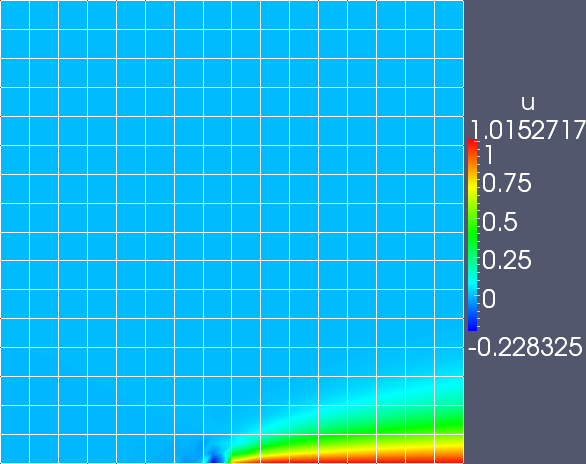
\includegraphics[width=2.5in]{dt10.png}}
\subfigure[$dt = .01$]{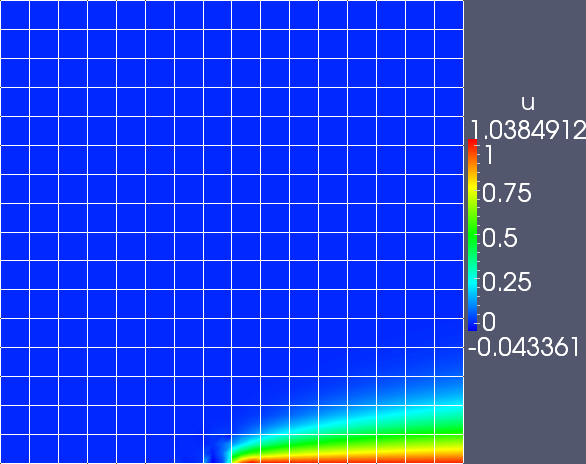
\includegraphics[width=2.5in]{dt100.png}}
\caption{Comparison of pseudo-timestepping to steady state for a convection-diffusion problem under two different sizes of timestep.}
\label{fig:dtComparison}
\end{figure}
This can be understood as the consequence of solving a ``moving target'' optimization problem -- our variational formulation and test norm for this problem are
\begin{align*}
\LRp{u_{i}, \frac{1}{dt}v}_{\L} + b\LRp{u_i,v} &= l(v) + \LRp{u_{i-1},\frac{1}{dt}v}_{\L}\\
\nor{\LRp{\tau,v}}_{V,dt}^2 &= \frac{1}{dt}\nor{v}_{\L}^2 + \nor{v}_V^2,
\end{align*}
where $\nor{\LRp{\tau,v}}_{V}$ is the test norm introduced in Section~\secref{sec:testNormSec}, and $b(u,v)$ and $l(v)$ are the bilinear form and load for the steady state form of the convection diffusion equation.  DPG solutions minimize the functional 
\[
J(u_i) = \sup_{v\in V} \frac{\LRp{u_{i}-u_{i-1}, \frac{1}{dt}v}_{\L} + b(u_i,v) - l(v)}{\LRp{\frac{1}{dt}\nor{v}_{\L}^2 + \nor{v}_V^2}^{\frac{1}{2}}}
\]
over a given mesh.  As $u_{i-1}\rightarrow u_{i}$, which we expect to happen as the pseudo-timestepping algorithm converges to steady state, the minimized functional becomes
\[
J(u_i) = \sup_{v\in V} \frac{b(u_i,v) - l(v)}{\LRp{\frac{1}{dt}\nor{v}_{\L}^2 + \nor{v}_V^2}^{\frac{1}{2}}}.
\]
While the transient portion of the residual disappears, a factor of $\frac{1}{dt}$ is still present in the test norm.\footnote{While the solution under smaller $dt$ appears to give visually higher quality results, we stress that simply adding the term $\frac{1}{dt}\nor{v}_{\L}$ to the test norm under the steady state version of the convection-diffusion equations does not achieve the same effect.  We are able to add this term without negative consequence due to the inclusion of the $\frac{u_i}{dt}$ term present in the variational formulation (see \cite{DPGrobustness,DPGrobustness2} for mathematical details).  Numerical experiments indicate that including $\alpha\nor{v}_{\L}$ in the test norm, where $\alpha > \frac{1}{dt}$, converges much more slowly to a fine-mesh reference solution than if $\alpha = \frac{1}{dt}$.}  Thus, we can expect that the nature of the steady state solution achieved through convergence of the pseudo-time algorithm can depend on the timestep $dt$.  We observe the same phenomena for analogous problems in compressible flow as well.  

\subsubsection{Adaptive time thresholding}

Adaptive timestepping (also known as pseudo-transient continuation) has been implemented successfully for problems in compressible flow \cite{BenKirk}. Typical adaptive time-stepping schemes modify the time-step based on some notion of the transient residual $R_i$ at timestep $i$, such that
\[
dt_{i+k} = \LRp{\frac{R_{i+k}}{R_i}}^r dt_i,
\]
where $r > 1$ dictates the rate of change of the timestep based on residual reduction, and $k$ indicates an integer interval at which to modify the timestep.  However, the minimum-residual nature of the DPG method and the ``moving target'' problem make the effectiveness of adaptive time-stepping schemes questionable.  

For our current experiments, we implement instead an adaptive time thresholding, where we adaptive decrease our convergence criterion based on the spatial energy error.  Recall that, under convergence of the pseudo-timestepping algorithm, the DPG energy error converges to the measure of the nonlinear residual in the dual norm.  We set convergence criterion for the pseudo-timestepping algorithm to be such that 
\[
\nor{e_{\rm time}}_V < \max \{\epsilon_t,\epsilon_{t,k}\},
\]
where $\epsilon_{t,k}$ is the tolerance at the $k$th refinement iteration, and $\epsilon_t < \epsilon_{t,k}$ is an absolute tolerance.  We initialize $\epsilon_{t,k}$ to $\epsilon_{t}$, then based on the energy error $\nor{u-u_h}_E$, we set 
\[
\epsilon_{t,k} = \alpha_t \nor{u-u_h}_E.
\]
Since the linearized error at a single timestep is composed of a sum of the linearization error, transient residual, and nonlinear residual, if the transient residual and linearization error are small, we expect that the nonlinear residual at that point will be sufficient to be an effective error indicator with which to drive adaptive mesh refinement.  In the following numerical experiments, $\alpha_t$ is set to $.005$.  

The aim of this adaptive thresholding is to relax the convergence criteria for solution of the nonlinear system at each refinement step such that the same refinement pattern is achieved with or without the use of adaptive time thresholding.  Numerical experiments seem to indicate that the same refinement pattern is produced with or without the implementation of this simple adaptive thresholding scheme, though wall-clock convergence times under adaptive thresholding are faster.  We hope to investigate both DPG-specific adaptive timestepping schemes and more advanced methods of balancing convergence criterion in the future.  

\subsection{Linear solver}

A clear choice for a linear solver under the ultra-weak variational formulation is static condensation, or the Schur-complement method. Given a block matrix structure of a stiffness matrix $K$, we can view the DPG system as
\[
Ku = \arr{A}{B}{B^T}{D}\vecttwo{u_{\rm flux}}{u_{\rm field}} = \vecttwo{f}{g} = l
\]
where $D$ has a block-diagonal structure, and $A$ and $D$ are both square matrices with $\dim{A} < \dim{D}$. This is due to the fact that, for the ultra-weak variational formulation (and for all HDG methods), the interior field degrees of freedom can be condensed out to yield a problem posed solely in terms of the coupled flux and trace degrees of freedom.  The system can be reduced to yield the condensed system
\[
\left(A-B D^{-1} B^T\right)u_{\rm flux} = f - B D^{-1} g
\]
where $D^{-1}$ can be inverted block-wise. Once the globally coupled flux and trace degrees of freedom are solved for, the field degrees of freedom can be reconstructed locally. An additional advantage of the above approach is that the Schur complement maintains the same sparsity pattern implied by the connectivity of the globally coupled flux and trace degrees of freedom.  Since the condensation process can be done locally, we can save memory by avoiding constructing the full stiffness matrix.

It has been shown that, unlike standard least-squares methods, DPG generates for the Poisson matrix a stiffness matrix with condition number $O(h^{-2})$ \cite{practicalDPG}. It is well known that, under standard finite element methods, if the condition number of the global stiffness matrix $K$ is $O(h^{-2})$, the condition number of the Schur complement is $O(h^{-1})$. Additionally, through either diagonal preconditioning or matrix equilibration, the condition number of the Schur complement can often be made significantly smaller than $O(h^{-1})$, and the positive-definiteness of the resulting system allows the use of iterative solvers in solving the condensed system.  Initial experiments indicate that, at least for quasi-uniform and low-order meshes, both algebraic multigrid and preconditioned conjugate gradients are able to solve the condensed system fairly rapidly.  We hope to experiment further with solvers for the condensed system, and to develop multigrid methods and preconditioners for adaptive and higher order meshes under DPG.  

\section{Test problems}

We applied the DPG method to two test problems in compressible flow -- flow over a flate plate, and flow over a compression ramp.  While the physics of both problems are fairly simple, they nonetheless display several features (shocks, singularities, boundary layers) that are computationally difficult to resolve without adaptivity.  Furthermore, the problems themselves are not usually solved without the aid of artificial or numerical diffusion and/or shock-capturing terms, which we eschew in our application of DPG to these model problems.

The numerical parameters used are as follows for:
\begin{itemize}
\item{DPG parameters:} $p = 2$ and $\Delta p = 2$ uniformly across the mesh. 
\item{Adaptivity parameters:} Energy threshold $\alpha$ for refinements is $\alpha = .4$ for the Carter flat plate example and $\alpha = .5$ for the Holden ramp example.  
\item{Time-stepping parameters:} Initial timestep $\Delta t = .1$, and initial tolerance for transient residual $\epsilon_t = 1e-7$.
\end{itemize}

Numerical experiments were run on a small cluster with 16 CPUs and 8GB memory, as well as on the Lonestar machine at the Texas Advanced Computing Center (TACC), using a varying number of cores, from 48 to 120 depending on problem geometry and parameters.  Experiments were done using the Camellia library \cite{Camellia}.
%Elements were partitioned using the Zoltan library of Trilinos \cite{ZoltanOverviewArticle}, using either a Hilbert space-filling curve or the REFTREE \cite{REFTREE} algorithm.  

\subsection{Numerical experiments: Carter flat plate}

The first problem of interest is the Carter flat plate problem \cite{Carter}. An infinitesmally thin flat plate disrupts a free stream flow, causing a shock to form at the tip of the plate, and a boundary layer forms and widens along the length of the plate.  

\begin{figure}
\centering
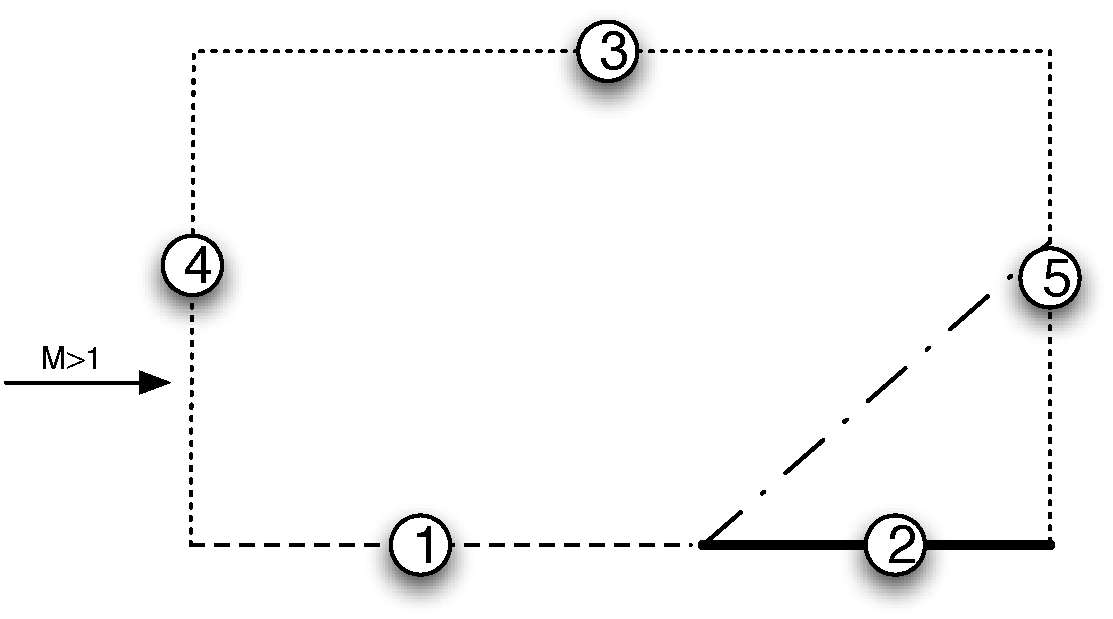
\includegraphics[width=3.5in]{flat_plate_BCs.pdf}
\caption{Carter flat plate problem.}
\end{figure}

\begin{enumerate}
\item \textbf{Symmetry boundary conditions:} $u_n = q_n = \pd{u_s}{n} = 0$. Here, this implies $u_2 = q_2 = \sigma_{12} = 0$. We impose the stress condition by noting that, for the flat plate geometry, if $u_2 = 0$, then at the top and bottom, with $n = (0,1)$, $\widehat{f}_{2,n} = \sigma_{12}$, and $\widehat{f}_{4,n} = q_2$ if $\sigma_{12}$ and $u_2 = 0$. They are applied here to the bottom free-stream boundary.
\item \textbf{Flat plate boundary conditions:} $u_1 = u_2 = 0$, and $T = T_w = \left[1+(\gamma-1)M_\infty^2/2\right] T_\infty = 2.8T_\infty$ (for Mach 3 flow). We impose these strongly on the trace variables $\widehat{u}_1, \widehat{u}_2, \widehat{T}$. 
\item \textbf{Symmetry boundary conditions} are applied also to the top free-stream boundary.
\item \textbf{Inflow boundary conditions:} free stream conditions are applied here to all four fluxes $\widehat{f}_{i,n}$.
\item \textbf{Outflow boundary conditions:} the exact boundary conditions to enforce here are not universally agreed on.  Many enforce $\pd{u_1}{n}=\pd{u_2}{n}=0$ and $\pd{T}{n} = 0$, while others enforce an outflow boundary condition only in regions where the flow is subsonic \cite{Demkowicz:1990:NFE:112271.112276}.  
We adopt a ``no boundary condition'' outflow condition, mimicing what is done in \cite{Shakib1991141}.%first introduced in \cite{FLD:FLD1650140506}. %A mathematical analysis and explanation of this boundary condition for standard $H^1$ elements is given in \cite{FLD:FLD505}. 
%An alternative boundary condition would be as follows: since $u_1$ and $u_2$ are not expected to be zero at these points, we can set $\widehat{f}_{2,n}$ and $\widehat{f}_{4,n}$ to their represented quantities using either the field variables from the background flow, or (in the case of pseudo-time stepping) the previous timestep's flux and field quantities. 
\end{enumerate}

We initialize our solution to
\[
\rho = 1,\qquad u_1= 1,\qquad u_2 = 0, \qquad T = 1%\frac{1}{\gamma(\gamma-1){\rm Ma}^2}
\]
which, we also take as the freestream values for the above variables, and is consistent with what was done by Demkowicz, Oden, and Rachowicz in \cite{Demkowicz1990275}. Stresses are set uniformly to zero.  We take the computational domain to be $\Omega = [0,2]\times[0,1]$. Under Dirichlet wall boundary conditions for all 3 traces $u_1$, $u_2$, and $T$, the solution develops a singularity in the density $\rho$ at the plate beginning, and both $T$ and $u_1$ form a boundary layer along the leading edge of the plate.  

\begin{figure}
\centering
\subfigure[$T$]{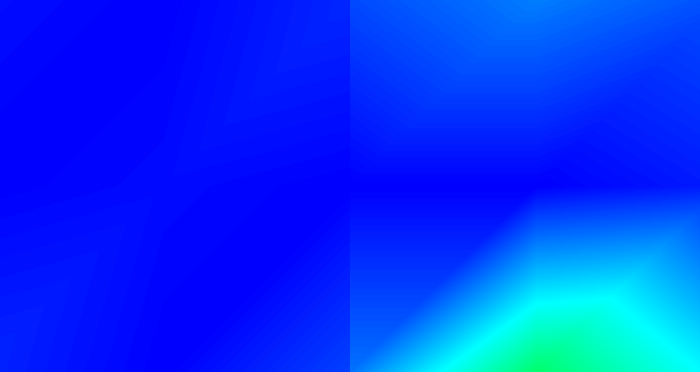
\includegraphics[width=2.5in]{T0.png}}
\subfigure[$u_1$]{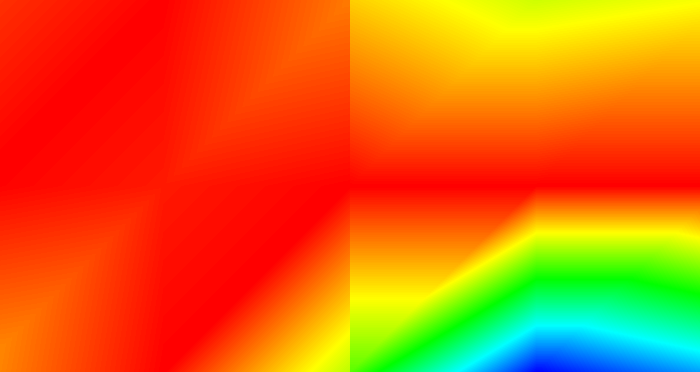
\includegraphics[width=2.5in]{u0.png}}
\caption{Converged solution on 2 cells.}
\label{fig:Re1000_2cells}
\end{figure}

We perform 10 steps of adaptive mesh refinement, beginning with a mesh of only two square elements.  The solution on this coarsest mesh is given in Figure~\ref{fig:Re1000_2cells}, and the final solutions after 10 refinement steps are given in Figure~\ref{fig:Re1000}.  For this specific example, we use only isotropic refinements.  

\begin{figure}
\centering
\subfigure[$\rho$]{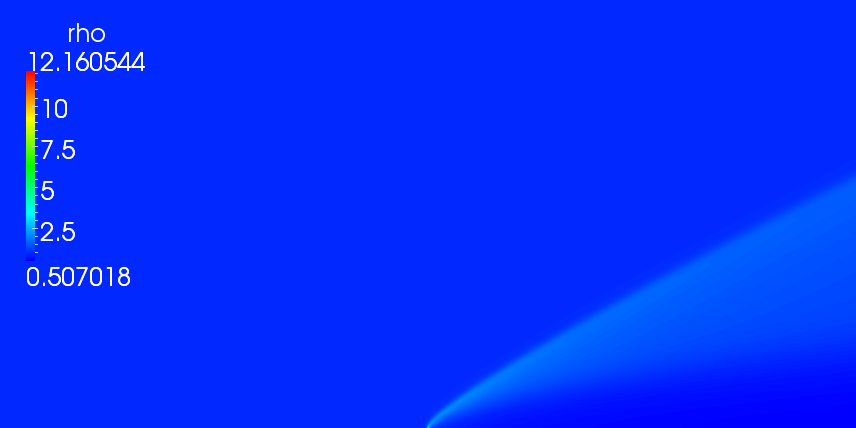
\includegraphics[width=2.8in]{rho.png}}
\subfigure[$u_1$]{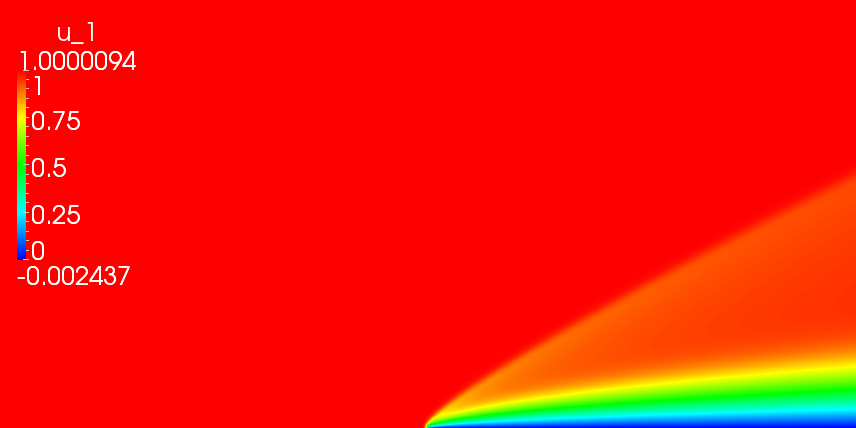
\includegraphics[width=2.8in]{u1.png}}
\subfigure[$u_2$]{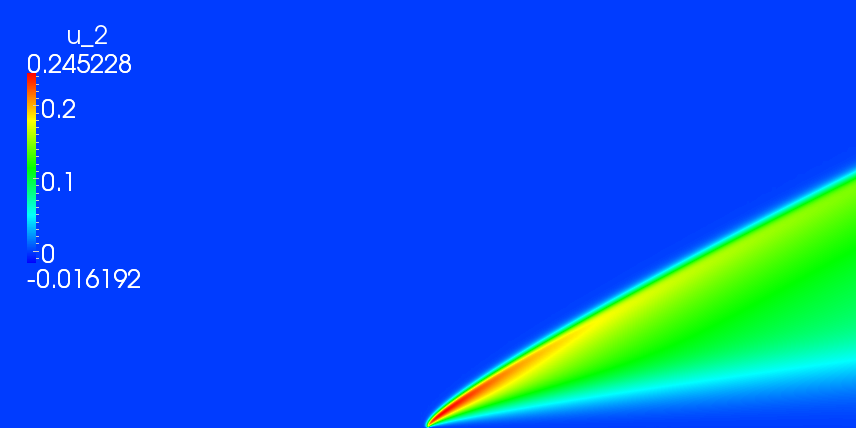
\includegraphics[width=2.8in]{u2.png}}
\subfigure[$T$]{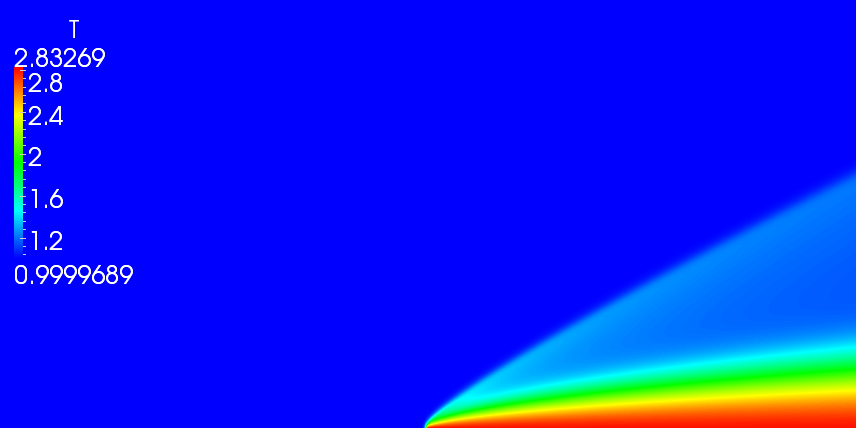
\includegraphics[width=2.8in]{T.png}}
\caption{Solutions after twelve refinements for $p=2$ and $\Reyn = 1000$, starting from a mesh of 2 elements.}
\label{fig:Re1000}
\end{figure}

Typical coarse meshes for adaptive CFD computations aim to resolve, at least to some degree, the features of the solution; often, physical features such as high gradients are used to drive refinement.  For feature-based adaptivity to be effective, coarse mesh solutions must be of sufficiently high quality to resolve basic solution features.  Often, artificial diffusion and shock capturing must also be applied in order to produce visually clean solutions on underresolved meshes.  In contrast to this, the residual-based approach of DPG is able to place refinements accurately and efficiently despite the underresolution of solution features.  

Figure~\ref{fig:Re1000_midRefs} shows snapshots of the third and sixth steps of adaptive mesh refinement.  The main contribution to energy error is at the plate tip -- due to the change in boundary condition across the point $(.5,0)$, the viscous stresses are singular at this point (this is analogous to the convection-diffusion plate example given earlier).  Underresolution of the stresses at this point results in some pollution effects slightly upstream of the beginning of the plate; however, once $h\approx {\rm Re}^{-1}$ near the plate edge, these pollution effects disappear.  We observe numerically that decreasing $dt$ also limits how far upstream of the plate edge this pollution effect travels.

\begin{figure}
\centering
\subfigure[Mesh, 4th refinement]{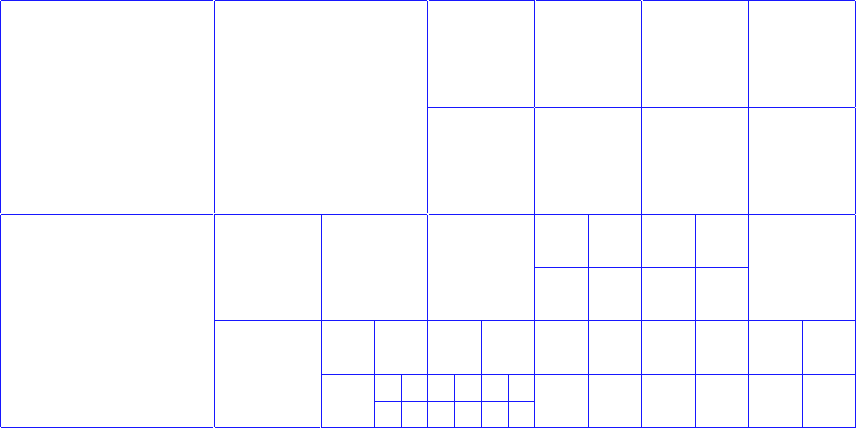
\includegraphics[width=2.85in]{mesh4.png}}
\subfigure[$T$, 4th refinement]{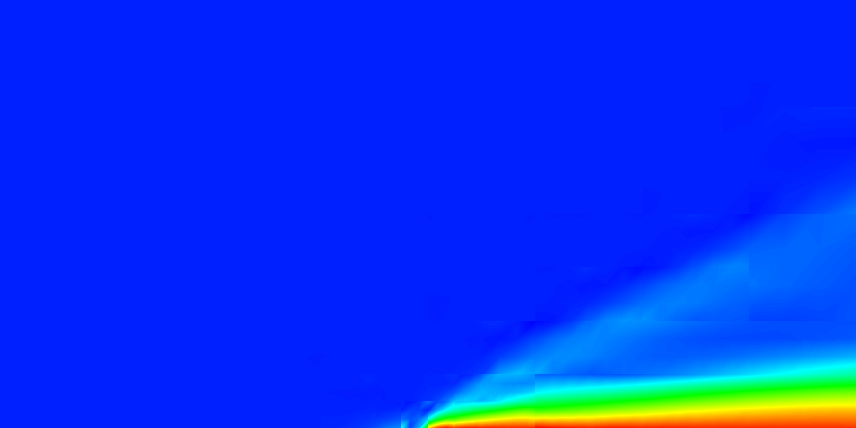
\includegraphics[width=2.85in]{T4.png}}
\subfigure[Mesh, 8th refinement]{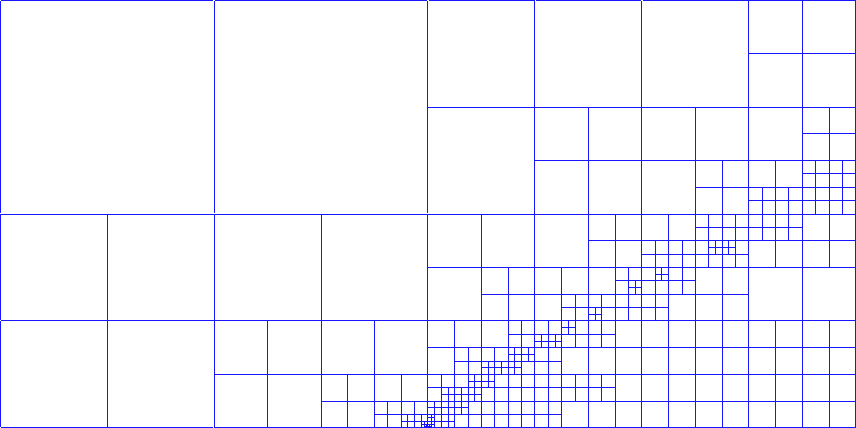
\includegraphics[width=2.85in]{mesh8.png}}
\subfigure[$T$, 8th refinement]{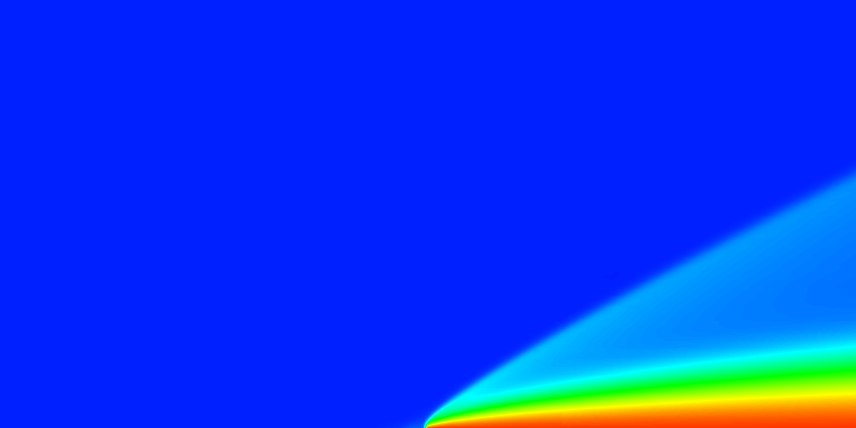
\includegraphics[width=2.85in]{T8.png}}
\caption{Snapshots of adaptive meshes and solutions for two different steps of adaptivity $\Reyn = 1000$.}
\label{fig:Re1000_midRefs}
\end{figure}

We observe numerically that $\rho$ also behaves singularly at the plate tip -- due to the presence of this strong singularity, the coloring of the wide range of values for $\rho$ in Figure~\ref{fig:Re1000} causes the solution to appears largely uniform, save for a flare up at the tip of the plate.  To better visualize density, $\rho$ is rescaled such that the features of the solution away from the singularity, as well as the final mesh after 10 refinement steps, are visible in Figure~\ref{fig:rhoScaled}.    

\begin{figure}
\centering
\subfigure[$\rho$]{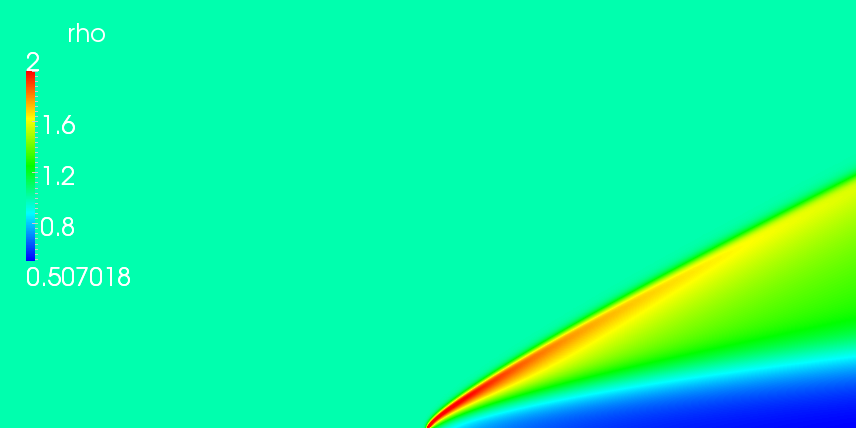
\includegraphics[width=2.8in]{rhoRescaled.png}}
\subfigure[Mesh]{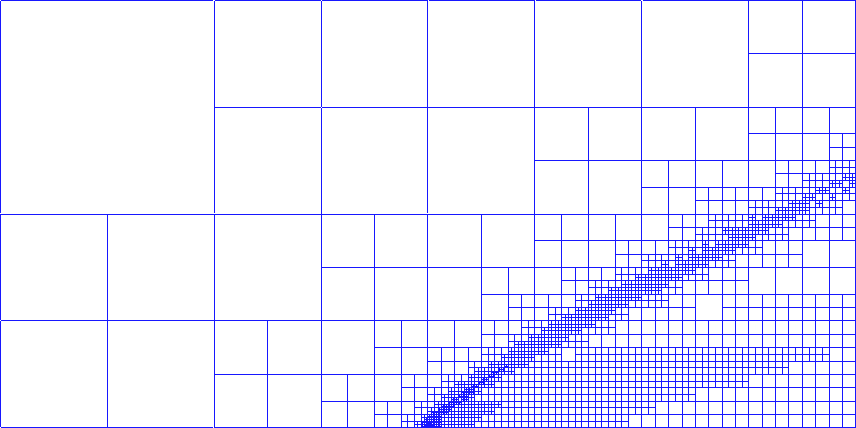
\includegraphics[width=2.8in]{mesh12.png}}
\caption{Rescaled solution for $\rho$ in the range $[\rho_{\min},2]$ and adaptive mesh after 12 refinement steps.}
\label{fig:rhoScaled}
\end{figure}

We can also zoom in on the plate tip to view the solution quality at the singular point.  Figure~\ref{fig:Re1000_zoom} demonstrates that the solution remains smooth and well-resolved at the plate tip, despite the presence of a singularity in the viscous stresses.%, and the fact that high order methods do not tend to resolve singularities as efficiently as low order methods \cite{hp1}.\cite{Optimal $hp$-adaptive strategies for elliptic problems with singularities result in meshes of lowest 

\begin{figure}
\centering
\subfigure[$\rho$]{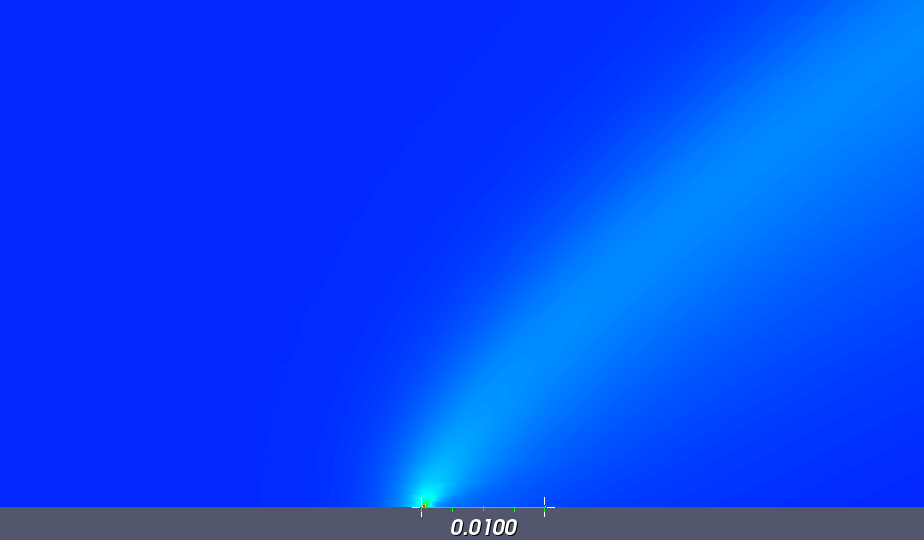
\includegraphics[scale=.23]{rhoZoom.png}}
\subfigure[$u_1$]{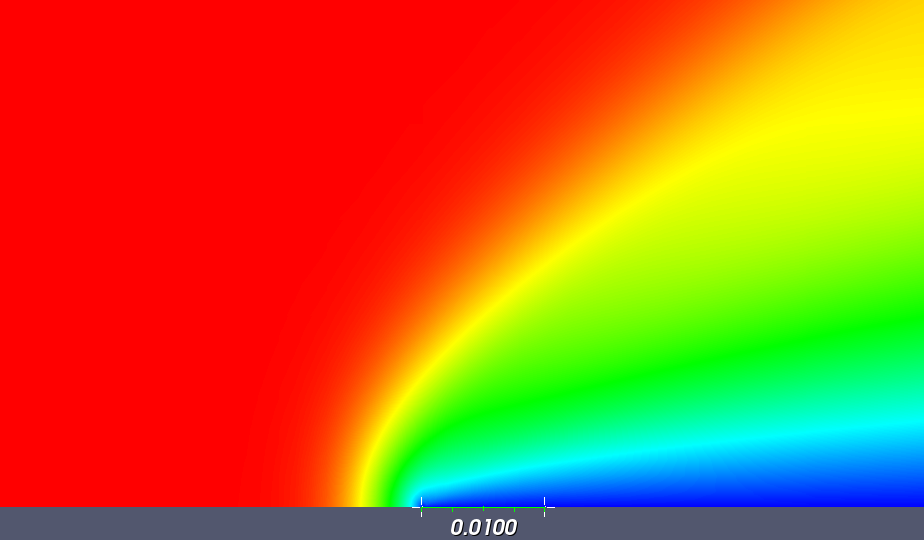
\includegraphics[scale=.23]{u1Zoom.png}}
\subfigure[$u_2$]{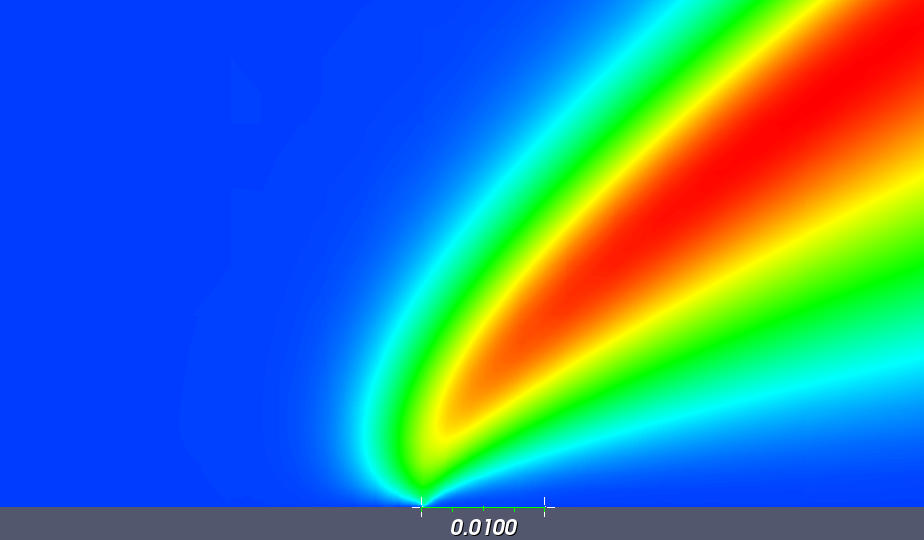
\includegraphics[scale=.23]{u2Zoom.png}}
\subfigure[$T$]{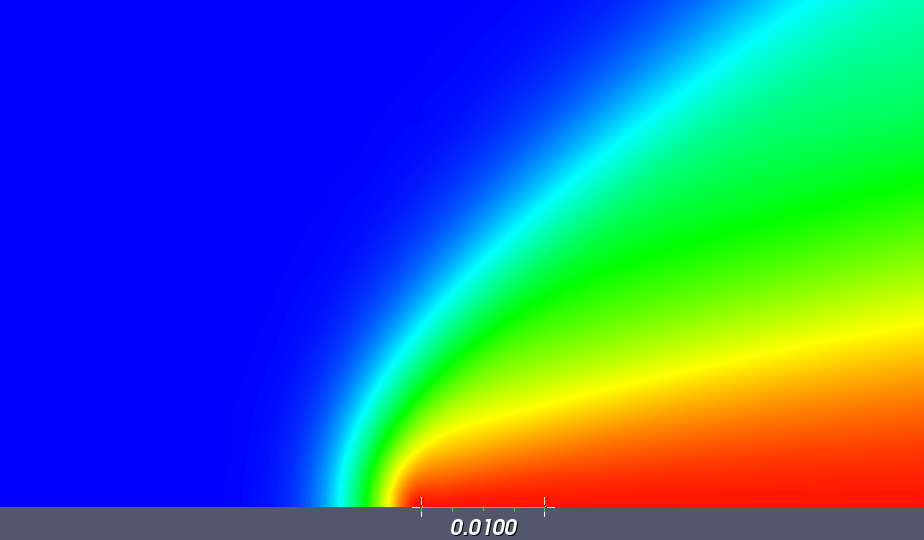
\includegraphics[scale=.23]{TZoom.png}}
\caption{Zoom of solutions at the beginning of the plate for $p=2$ and $\Reyn = 1000$.}
\label{fig:Re1000_zoom} 
\end{figure}

We increased the Reynolds number to $10,000$ to assess the behavior of DPG for higher Reynolds numbers.  However, we found it necessary to modify the method in several ways in order to achieve satisfactory results.  

First, we implemented a line search algorithm to enforce positivity of both temperature and density, which are physically defined to be positive quantities.  Given updates $\triangle \rho$ and $\triangle T$, we update our previous solution by setting 
\begin{align*}
\rho \coloneqq \rho + \alpha_{\rm line}\triangle \rho \\
T \coloneqq T + \alpha_{\rm line}\triangle T,
\end{align*}
where $\alpha_{\rm line}$ is chosen, for some $\delta > 0$, such that
\begin{align*}
\rho + \alpha_{\rm line}\triangle \rho - \delta = 0\\
T + \alpha_{\rm line}\triangle T  - \delta = 0.
\end{align*}
Since the addition of a line search can slow the convergence of a nonlinear algorithm, we incorporate also a Newton iteration at each timestep to effectively solve the nonlinear system at each timestep.  We consider $\nor{\triangle U}_E < \epsilon_{\rm Newton}$ to be our condition for convergence of the Newton iteration, though we also limit the number of allowed Newton steps for computational efficiency.  The full solver algorithm is given in Algorithm~\ref{fig:algorithm}.  
\begin{algorithm}                      % enter the algorithm environment
\caption{Calculate $y = x^n$}          % give the algorithm a caption
\label{alg1}                           % and a label for \ref{} commands later in the document
\begin{algorithmic}                    % enter the algorithmic environment
\FOR{ number of refinement steps } 
    \WHILE{ $R_{\rm time} > \epsilon_t$}
        \STATE k = 0
        \WHILE{$\nor{\triangle U}_E > \epsilon_{\rm Newton}$ and $k <$ maximum Newton steps}
            \STATE Solve for $\triangle U$, determine $\alpha_{\rm line}$.  
            \STATE $U \coloneqq U + \alpha_{\rm line}\triangle U$.  
            \STATE k = k+1
        \ENDWHILE
        \STATE Increment timestep.  
    \ENDWHILE
    \STATE Compute energy error and refine based on a greedy refinement algorithm.
    \STATE Set $\epsilon_t = \alpha_t \nor{u-u_h}_E$.    
\ENDFOR
\end{algorithmic}
\caption{Pseudo-timetepping adaptive algorithm with line search.}
\label{fig:algorithm}
\end{algorithm}
For higher Reynolds numbers and highly refined meshes, the solution update exhibits large oscillations, such that the solution at a timestep can become negative, under which the pseudo-timestepping algorithm can stall or even diverge.\footnote{We note that these large oscillations mimic experiences in 1D as well, where the linearized solution was shown to exhibit sharp gradients near shocks that did not disappear, even with additional mesh refinement, indicating that the presence of such overshoots and undershoots is a consequence of the linearization, as opposed to the stability of the discretization \cite{NS_DPG1D}. This is discussed in more detail in Section~\secref{sec:oscillations}.  

We note also that theory developed in \cite{DPGrobustness2} for the convection-diffusion problem assumes a smooth convection field.  However, under linearization of the Burgers' and Navier-Stokes equations, the solution around which we linearize dictates the convection field, and can display large gradients.  While we have not observed issues in the Burgers' equation related to this, we hope to revisit the analysis done in \cite{DPGrobustness2} and generalize it for convection fields with large gradients.}.  However, we have observed that requiring a strictly positive solution appears to be too restrictive a constraint for some meshes; the use of line search does not appear to be necessary for convergence of the pseudo-timestepping algorithm on coarser meshes (until the 10th refinement iteration, or $h< .001$).  

Finally, we implement an ``effective'' CFL number; though implicit time integration schemes are unconditionally stable (compared to explicit schemes), a CFL condition relating the size of the time increment to the (minimum) mesh size is often still used in practice to improve convergence speed and stability of the numerical scheme \cite{Shakib1991141}.   Our CFL number is chosen to be 64.  We note that this CFL number is implemented for non-standard reasons.  In fact, DPG is able to solve the steady-state system directly without the use of pseudo-timestepping (direct Newton iteration).  However, as noted previously, the size of the timestep under which pseudo-timestepping converges greatly affects the qualitative nature of the solution.  Figure~\ref{fig:dtCompare} demonstrates the difference between convergence at large and small timesteps -- for $dt$ large relative to the mesh size, the solution experiences upstream ``pollution'' effects.  
\begin{figure}
\centering
\subfigure[$dt = \infty$ (Direct Newton)]{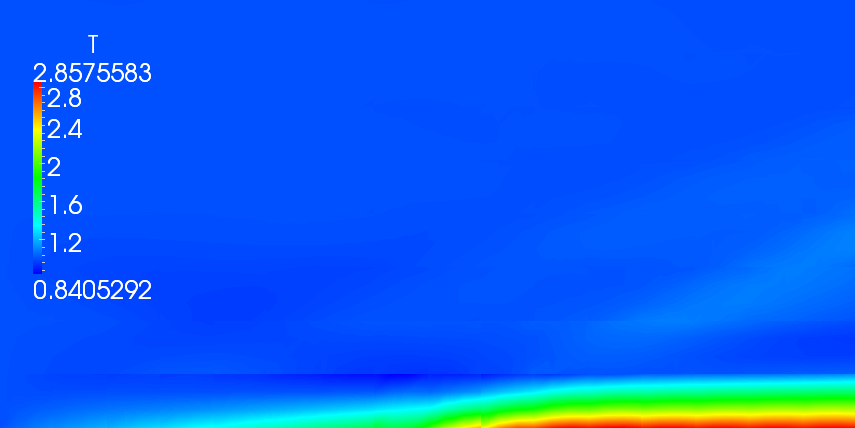
\includegraphics[width=2.8in]{dtInf.png}}
\subfigure[$dt = 1.0$]{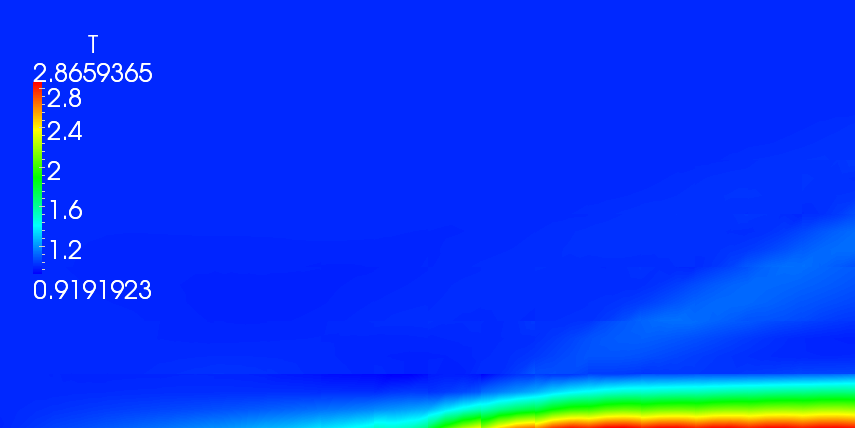
\includegraphics[width=2.8in]{dtOne.png}}
\subfigure[$dt = .1$]{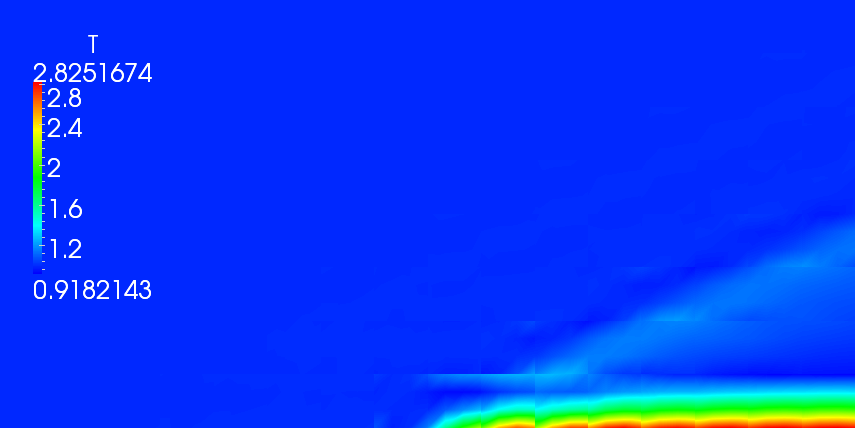
\includegraphics[width=2.8in]{dtTenth.png}}
\caption{Steady state solutions for ${\rm Re} = 10,000$ under three different timesteps on a $16\times 8$ uniform mesh.}
\label{fig:dtCompare}
\end{figure}
Due to the upstream ``pollution'' present in the solution for $dt \geq 1$, the adaptive mesh refinement algorithm tends to add extraneous refinements on elements adjacent to the boundary $y = 0$, $x\in (0,1)$.  Decreasing the timestep alleviates this issue somewhat; however, an overly small timestep requires a large number of iterations to converge.  The implementation of an effective CFL number aims to balance the size of the timestep with the mesh size.\footnote{An additional reason for the implementation of an effective CFL number is the conditioning of the local problem, which was discussed for the convection-dominated diffusion problem in \cite{DPG3}.  The main problem concerning conditioning of local problems is the way that different test terms behave as a function of local element size.  We illustrate this using the element Sobolev norm $\nor{v}_{H^1(K)} = \nor{v}_{\L} + \nor{\grad v}_{\L}$ -- $\nor{v}_{\L} = O(h^2)$ (where $h$ is the element size), while $\nor{\grad v}_{\L} = O(1)$.  Thus, as $h\rightarrow 0$, the Sobolev norm over a single element approaches the Sobolev seminorm and loses positive definiteness, resulting in a highly ill-conditioned system to solve.  The addition of a first-order pseudo-timestepping term allows us to increase the relative magnitude of $\nor{v}_{\L}$ with respect to $\nor{\grad v}_{\L}$ and avoid conditioning issues while maintaining robustness of the method.}  

We note that, even with all of the above modifications, the pseudo-timetepping adaptive algorithm with line search would sometimes failed to converge below $\epsilon_t$ for ${\rm Re} \geq 10,000$.  Figure~\ref{fig:nonconvergence} shows a plot of the transient residual after the 14th refinement step; while the residual initially decreases, it stalls at about $R_{\rm time} \approx 10^{-4}$.  
\begin{figure}
\centering
\subfigure[Non-convergence]{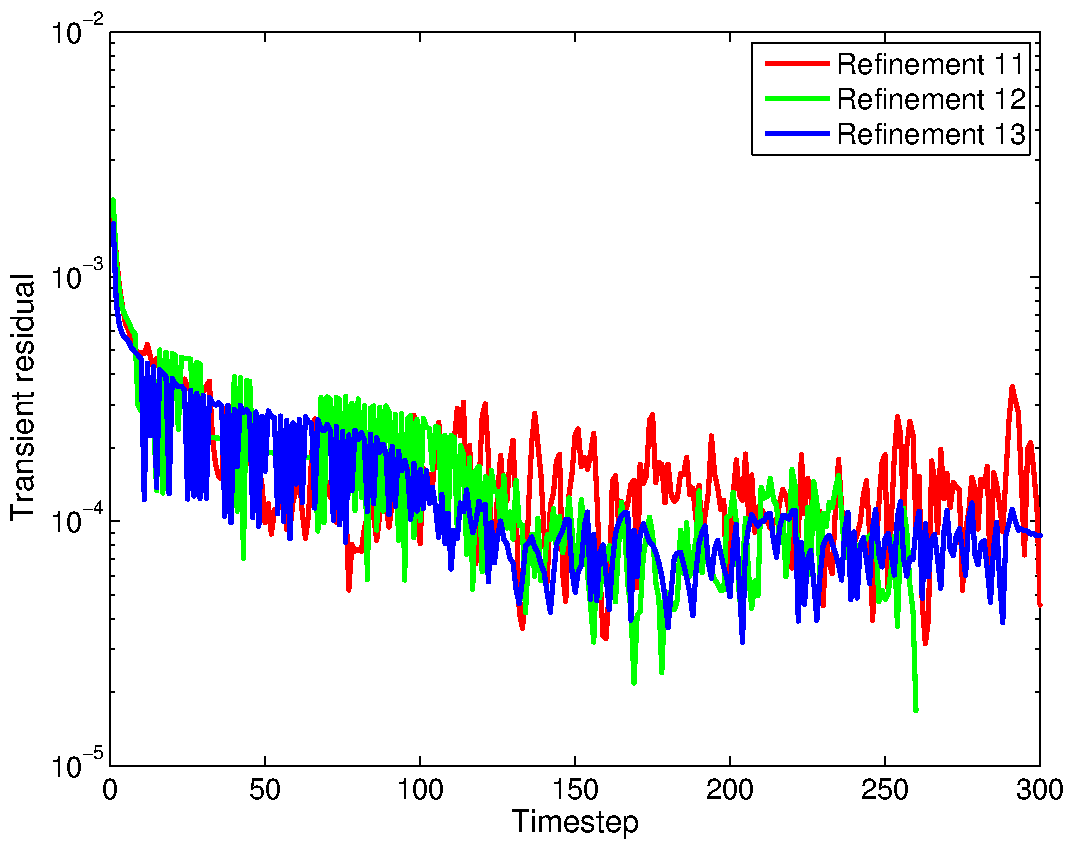
\includegraphics[width=2.5in]{oscillations1.pdf}}
\subfigure[Recovery of convergence]{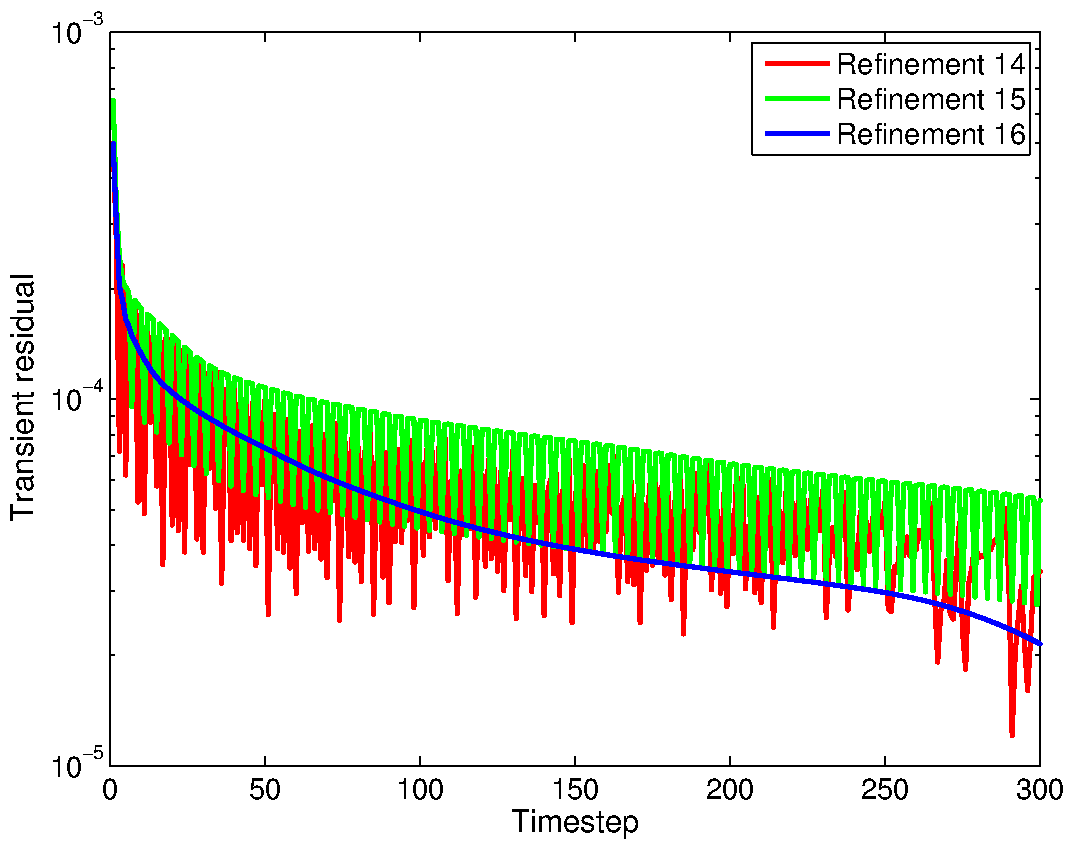
\includegraphics[width=2.5in]{oscillations2.pdf}}
\caption{Stalling and recovery of the pseudo-timestep iteration for $\Reyn = 10000$.}
\label{fig:nonconvergence}
\end{figure}
An examination of the difference in the solutions between the final and $125$th timesteps shows that the nonconvergence of the transient residual is due to oscillations in the solution (primarily in $\rho$) slightly upstream to the plate edge.  Visually, the solution converges everywhere else, save for this area.  Such behavior is also observed in \cite{BenKirk}, where, at the change in boundary conditions between the free stream and flat plate, an oscillation was observed in the solution which prevented convergence of his pseudo-time algorithm.  His oscillations are of smaller magnitude ($O\LRp{10^{-6}}$ as opposed to $O\LRp{10^{-4}}$), which may be the result of several differences between the methods presented.\footnote{Apart from the use of a standard Galerkin (continuous as opposed to discontinuous Galerkin) formulation, Kirk's approach differed from ours in the use of linear elements and the addition of artificial diffusion shock-capturing terms, both of which could explain the lower point at which error stagnates. Reasons for this loss of convergence in the pre-asymptotic range should be explored further.}  However, we note that, under additional refinements and increased resolution of the solution, the transient residual once again decreases in a smooth monotonic fashion, as shown in Figure~\ref{fig:nonconvergence}. 

\begin{figure}
\centering
\subfigure[$\rho$]{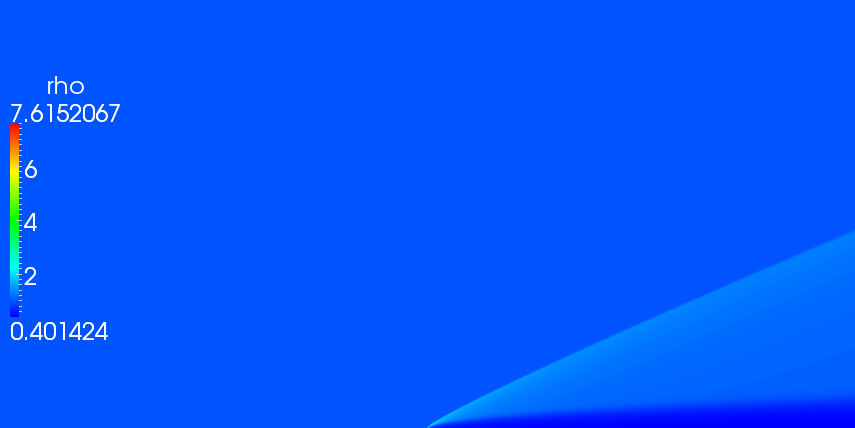
\includegraphics[width=2.8in]{rhoRe4Plate.png}}
\subfigure[$u_1$]{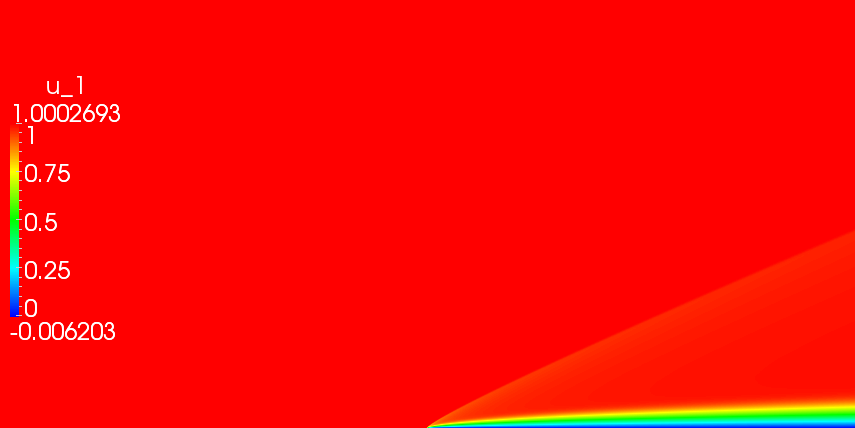
\includegraphics[width=2.8in]{u1Re4Plate.png}}
\subfigure[$u_2$]{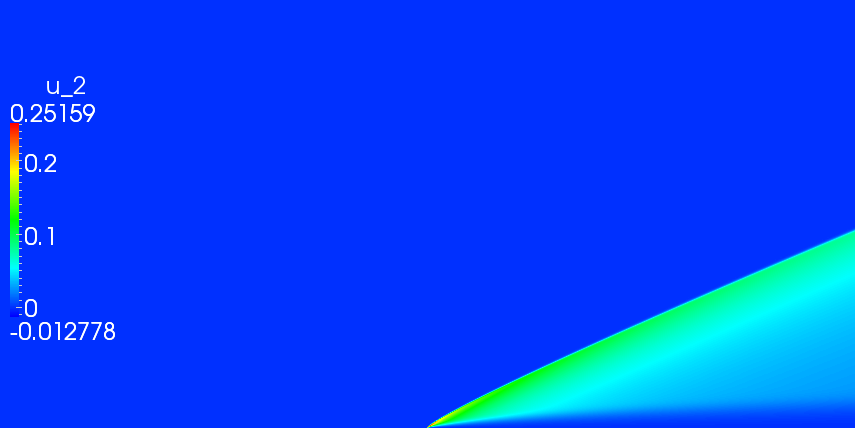
\includegraphics[width=2.8in]{u2Re4Plate.png}}
\subfigure[$T$]{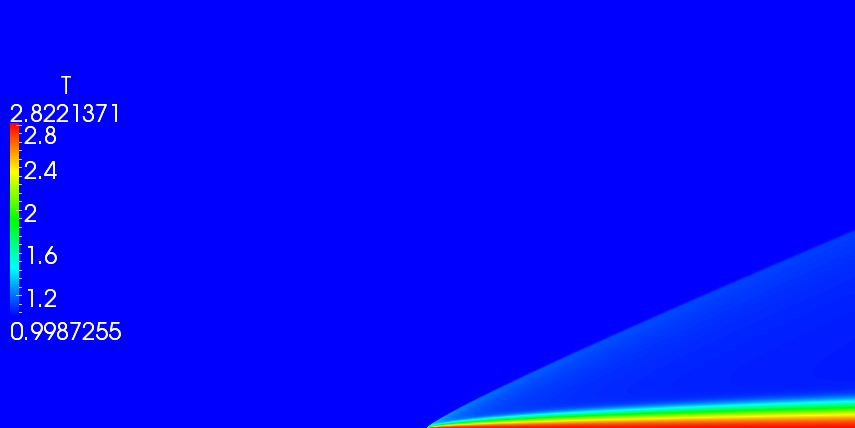
\includegraphics[width=2.8in]{TRe4Plate.png}}
\caption{Solutions after 18 refinements for $p=2$ and $\Reyn = 10000$.}
\label{fig:Re10000}
\end{figure}

For additional computational efficiency, we also implemented an anisotropic refinement scheme.  In 2D, the boundary layer is a primarily 1D phenomena, which we expect to be far better resolved by anisotropic refinement than by isotropic refinement.  We experimented first using the scheme described in Section~\secref{sec:aniso} as an anisotropy indicator; however, the anisotropic scheme appeared to be too conservative near the boundary layer, placing primarily isotropic refinements.  We modified our scheme in two ways -- first, we incorporated spatially variable thresholding.  Typically, anisotropic refinement in the $x$ direction is chosen if $e_{x,K} > \epsilon_r e_{y,K}$ (and vice versa for anisotropic refinement in the $y$-direction), where $e_{x_i,K}$ is the error in the $x_i$ direction.  We set $\epsilon_r = \epsilon_{r,K}$; in other words, we allow our anisotropic threshold to vary element-by-element, and decrease it from $\epsilon_r= 10$ to $\epsilon_{r,K} = 2.5$ for elements adjacent to the wall upon which the boundary layer forms.  Additionally, since the boundary layer typically displays rapid variation in the $y$-direction (the direction orthogonal to the wall), we relax the condition under which a vertically cut anisotropic refinement occurs to
\[
2 e_{y,K} > \epsilon_{r,K} e_{x,K}.
\]
Despite the artificial modification of the anisotropic refinement scheme, the resulting meshes still resolve boundary layer solutions more efficiently than isotropic refinements.  We hope to investigate reasons for the ineffectiveness of the pure anisotropic scheme for the compressible Navier-Stokes equations in future research.  

\begin{figure}
\centering
\subfigure[$\rho$]{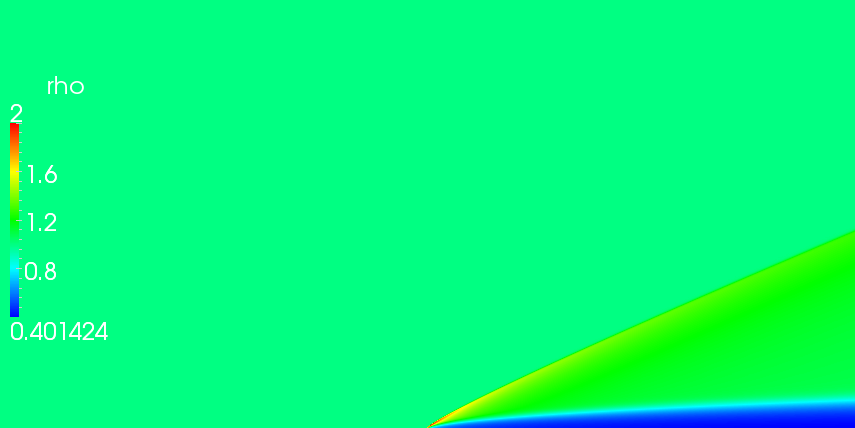
\includegraphics[width=2.8in]{rhoRescaledRe4Plate.png}}
\subfigure[Mesh]{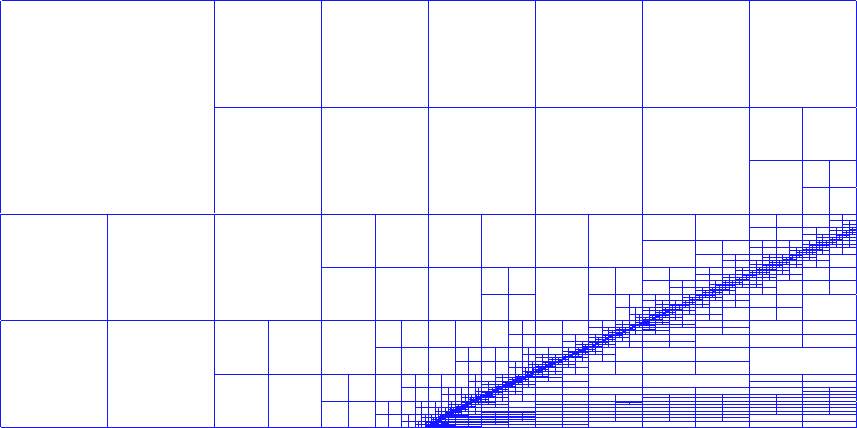
\includegraphics[width=2.8in]{meshRe4Plate.png}}
\caption{Rescaled solution for $\rho$ in the range $[\rho_{\min},2]$ and adapted mesh.}
\label{fig:rhoScaled}
\end{figure}

\begin{figure}
\centering
\subfigure[$\rho$]{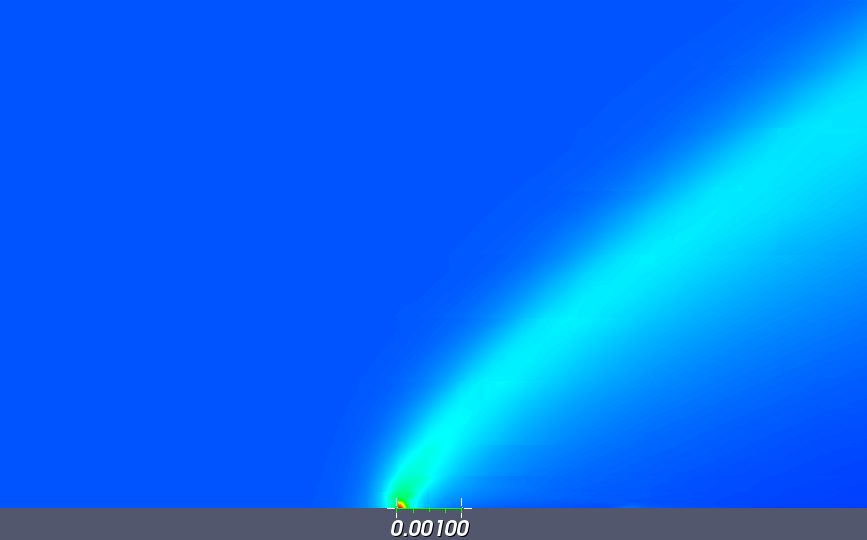
\includegraphics[width=2.8in]{rhoZoomRe4Plate.png}}
\subfigure[$u_1$]{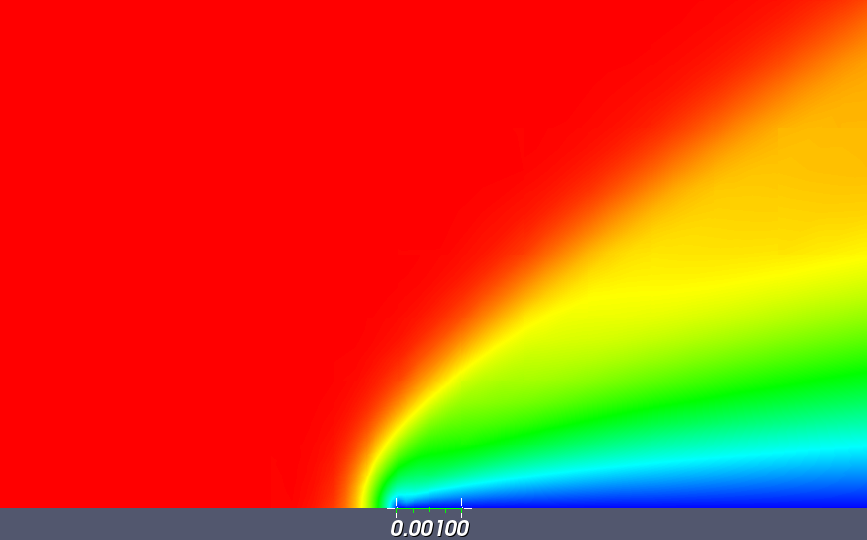
\includegraphics[width=2.8in]{u1ZoomRe4Plate.png}}
\subfigure[$u_2$]{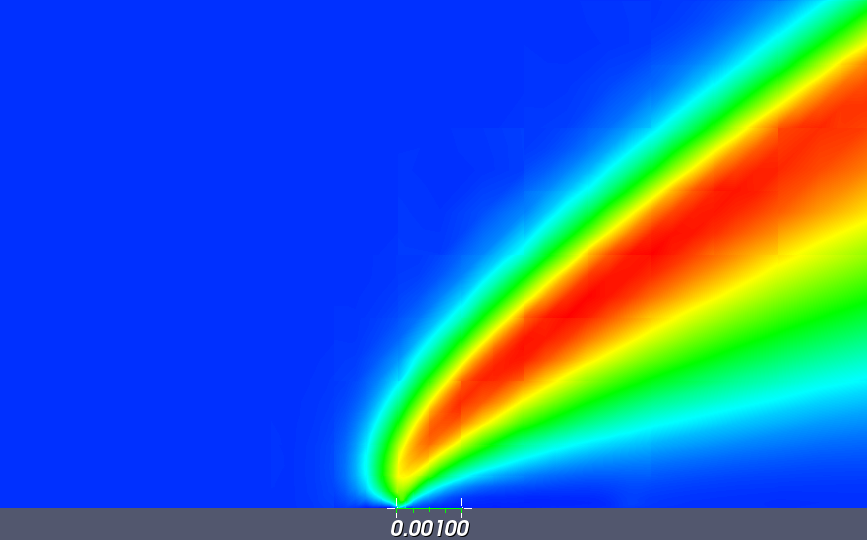
\includegraphics[width=2.8in]{u2ZoomRe4Plate.png}}
\subfigure[$T$]{\includegraphics[width=2.8in]{TZoomRe4Plate.png}}
\caption{Zoom of solutions at the beginning of the plate for $p=2$ and $\Reyn = 10000$.}
\label{fig:Re1e4Zoom}
\end{figure}

We note that the resolution of the solution near the plate edge in Figure~\ref{fig:Re1e4Zoom} for Reynolds number 10000 is qualitatively rougher than that for Reynolds 1000 in Figure~\ref{fig:Re1000_zoom}; this is due to the greedy refinement algorithm emphasizing refinements most strongly at the singular point and not in shock resolution, as well as the fact that at a higher Reynolds number, the shock width is thinner and more difficult to resolve.  Further refinement steps improve resolution of the shock features.  

%\begin{figure}[!h]
%\centering
%\subfigure[${\rm Re} = 1000$]{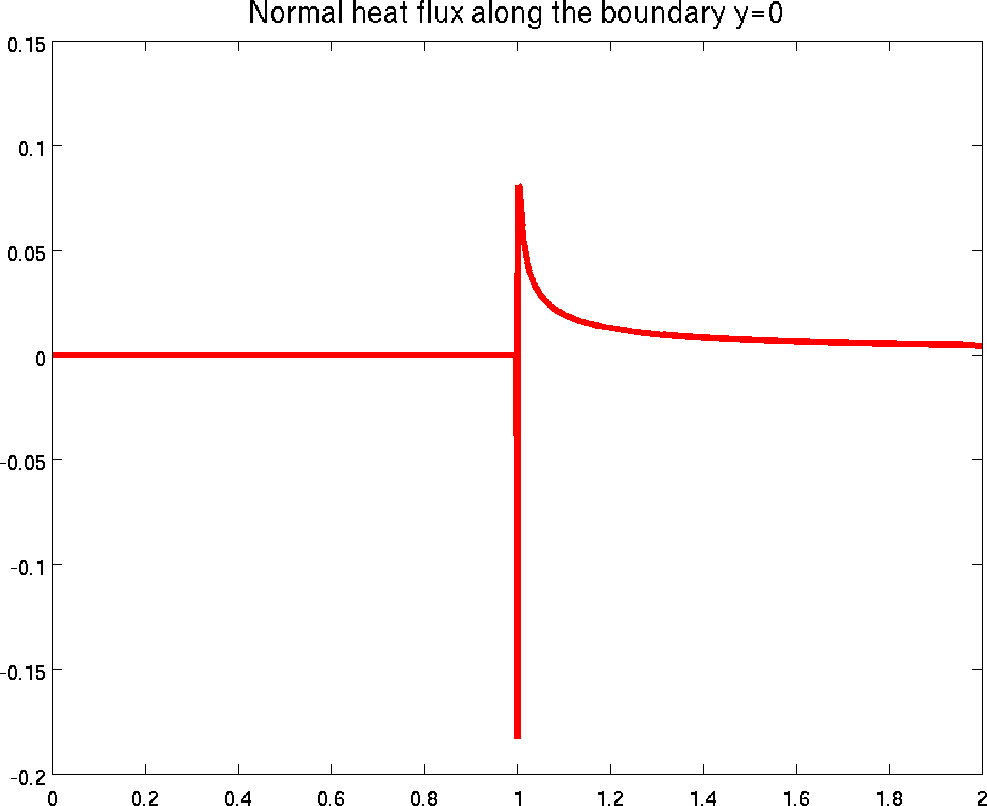
\includegraphics[scale=.5]{figs/Re1000p2/heatflux.png}}
%\subfigure[${\rm Re} = 10000$]{\includegraphics[scale=.3]{figs/Re1e5/q2line.png}}
%\caption{Heat flux at the bottom boundary.}
%\end{figure}

\subsection{Holden ramp problem}

Our second problem is a modified version of the Holden ramp problem, which models supersonic/hypersonic flow over a compression corner (the geometry of which is given in Figure~\ref{fig:holdenCartoon}).  Similarly to the Carter flat plate problem, a flat plate disrupts the flow and forms a weak shock at the plate tip due to viscous effects and no-slip boundary conditions.  The boundary layer grows down the plate edge, deflecting upwards due to the presence of the compression corner.  A stronger shock forms slightly upstream of the compression corner in order to deflect the incoming supersonic flow, and is a common test problem for adaptive finite element methods for compressible flow \cite{Rachowicz1997231,Barter,BenKirk}.  

\begin{figure}
\centering
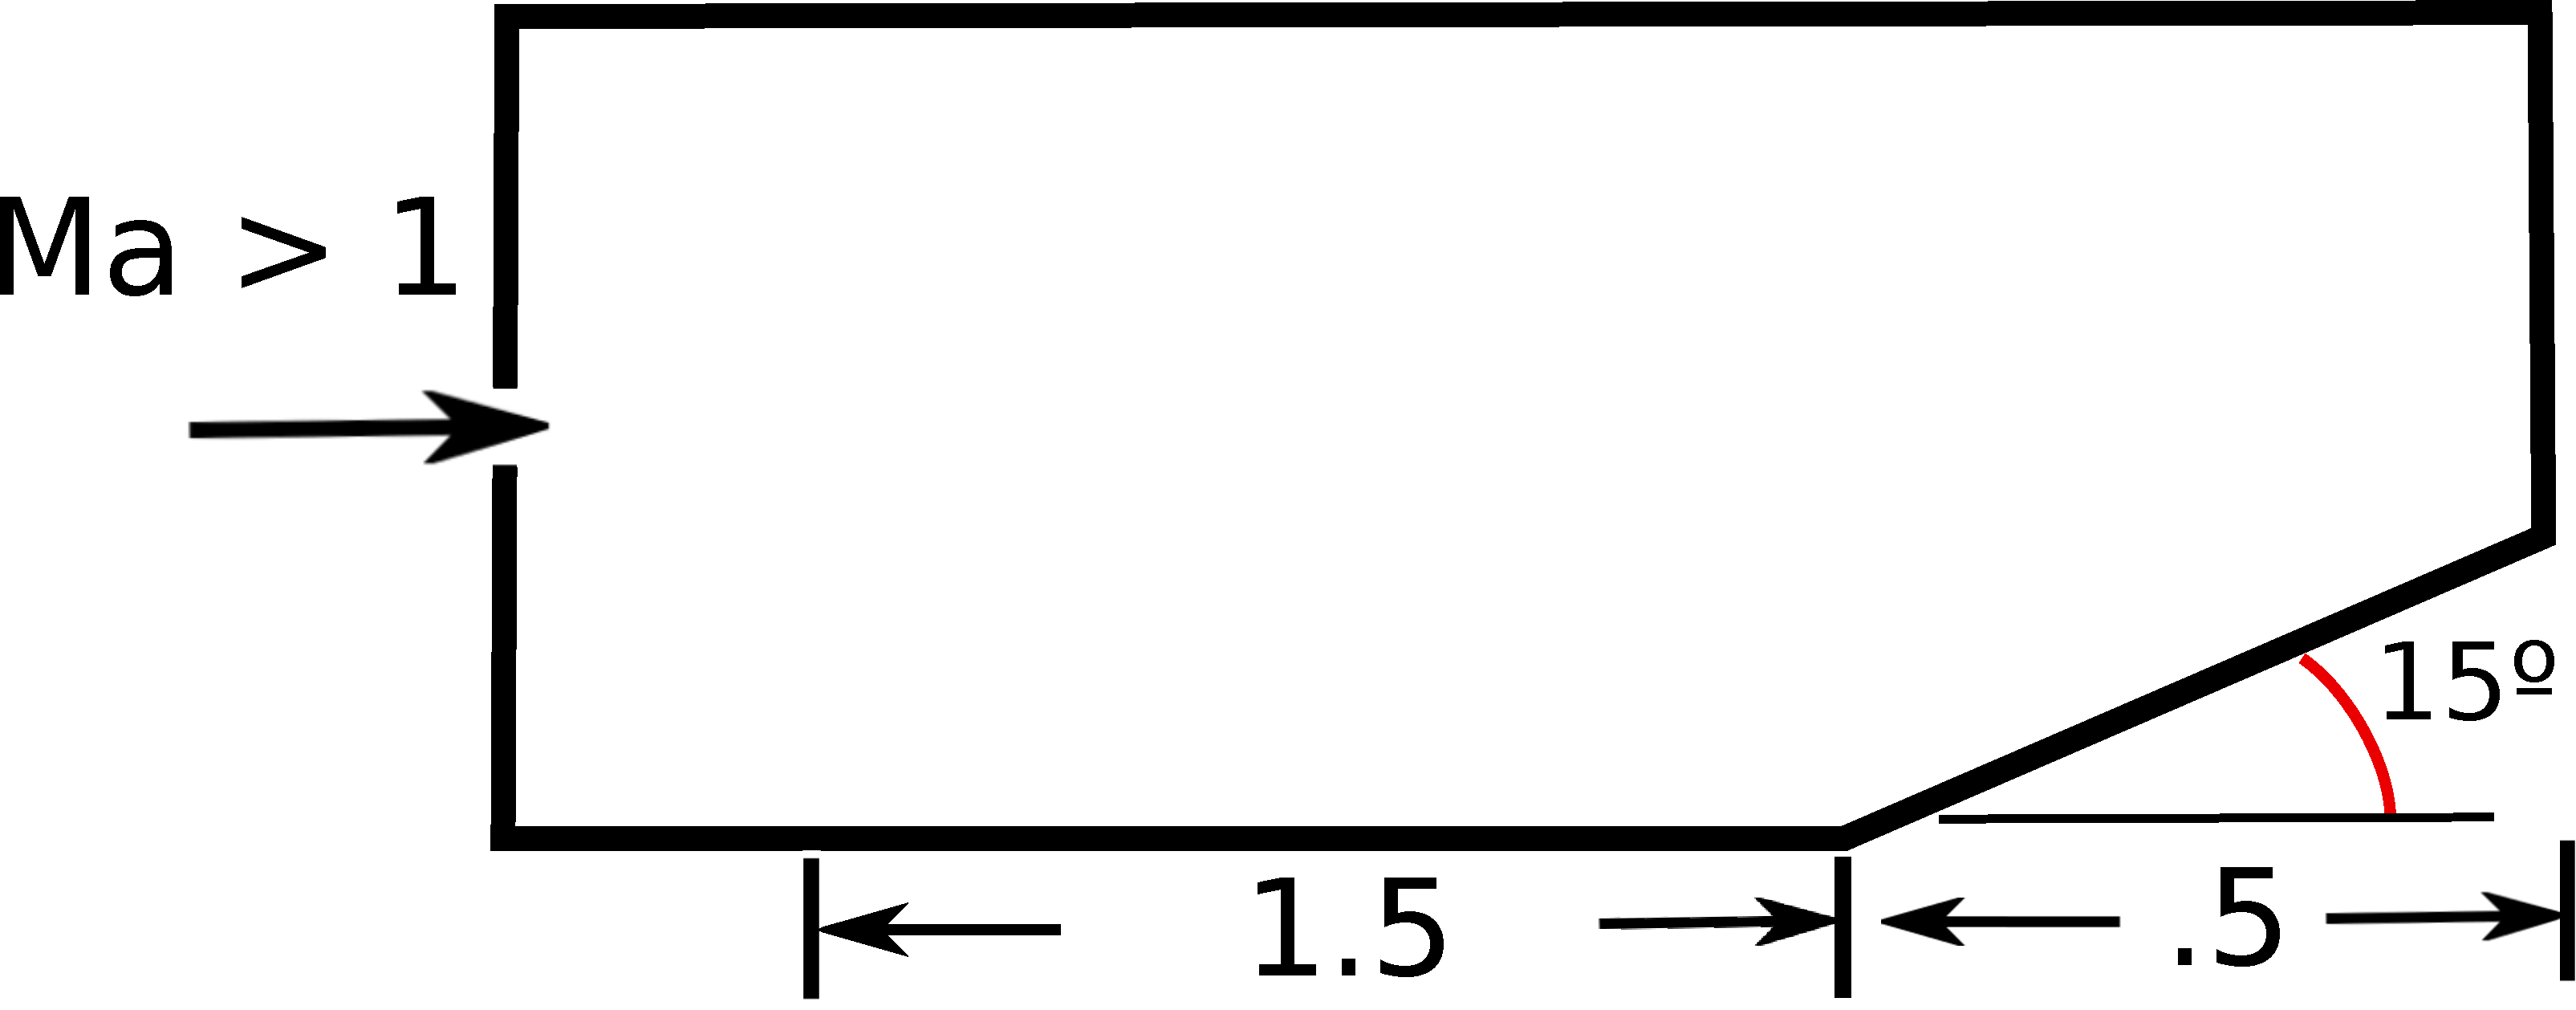
\includegraphics[width=4in]{holden.pdf}
\caption{A modification of the Holden ramp/compression corner problem.}
\label{fig:holdenCartoon}
\end{figure}

The original plate length is given to be .442, while the ramp length is given to be .269. We have modified the problem slightly in order to exactly represent the boundary conditions on a coarse mesh while keeping the ratio of plate length to ramp length roughly the same. Similarly to the Carter flat plate, we start out with a very coarse $2 \times 3$ mesh of 6 elements.  We initialize our solution to the freestream values
\[
\rho_{\infty} = 1,\qquad u_{1,\infty}= 1,\qquad u_{2,\infty} = 0, \qquad T_{\infty} = 1
\]
and again set stresses uniformly to zero.   

\begin{figure}
\centering
\subfigure[$\rho$ rescaled]{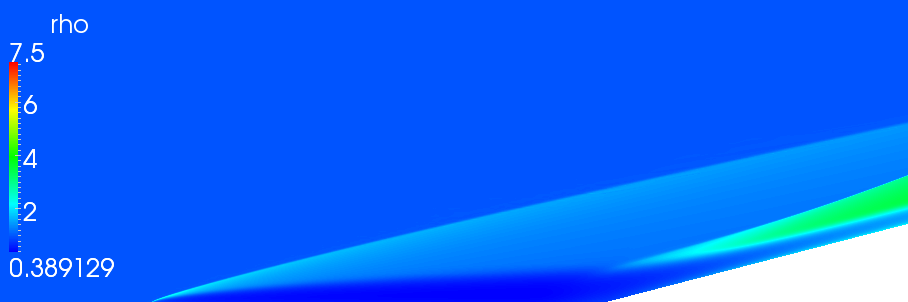
\includegraphics[width = 2.9in]{rhoRescaledMa6Ramp.png}}
\subfigure[$u_1$]{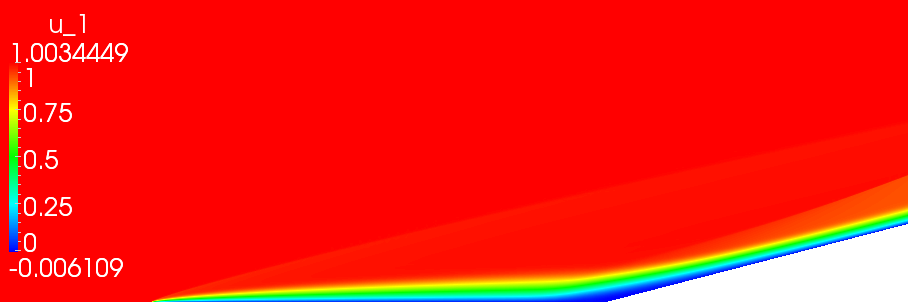
\includegraphics[width = 2.9in]{u1Ma6Ramp.png}}
\subfigure[$u_2$]{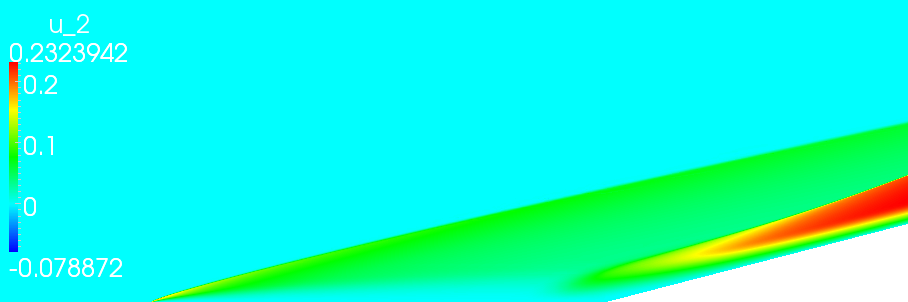
\includegraphics[width = 2.9in]{u2Ma6Ramp.png}}
\subfigure[$T$]{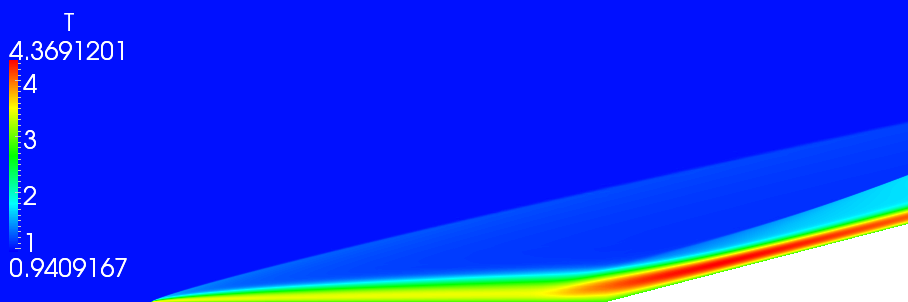
\includegraphics[width = 2.9in]{TMa6Ramp.png}}
\subfigure[Mesh]{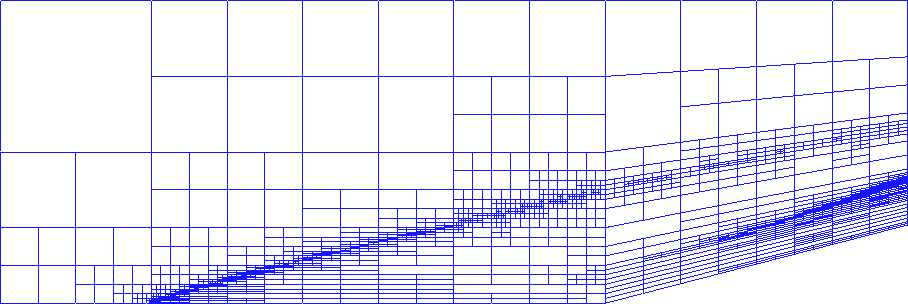
\includegraphics[width = 5.5in]{meshMa6Ramp.png}}
\caption{Solutions and adaptive mesh for ${\rm Ma} = 6$ and $\Reyn = 10000$.}
\label{fig:holdenMa6}
\end{figure}

We first solve under Mach 6 flow.\footnote{The increase in Mach number is to change the angle of the shock; under the current setup, Mach 3 flow produced a shock which reflected off the top boundary $y = 1$  We note that the effect of Mach number under our nondimensionalization of choice is to decrease the thermal diffusivity constant $\kappa$ relative to the viscosities $\mu$ and $\lambda$.} and Reynolds number of 10,000, or a Reynolds number of 33,936 if measured with respect to the original plate length of .442.  The wall temperature is set to $T_{w} = 2.8T_{\infty}$, identically to the flat plate problem.  24 mesh refinements were performed, resulting in a final mesh of 1858 elements.  Figure~\ref{fig:holdenMa6} shows both solution values and final adaptive mesh.  Due to a large maximum value of $\rho_{\max} = 14.1538$ at the plate tip, the resulting solution for $\rho$ is scaled to better show qualitative features of the flow.  The presence of the second shock deflecting the incoming supersonic flow at the ramp is clearly seen in both the solutions and the adaptive mesh refinements.  

\begin{figure}
\centering
\subfigure[Initial mesh]{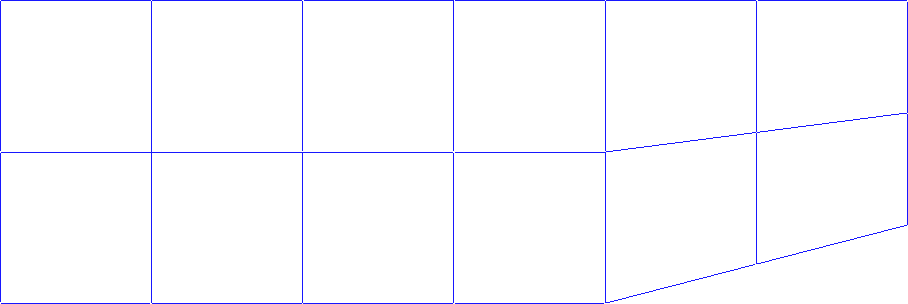
\includegraphics[width = 2.9in]{rampMesh0.png}}
\subfigure[6 refinements]{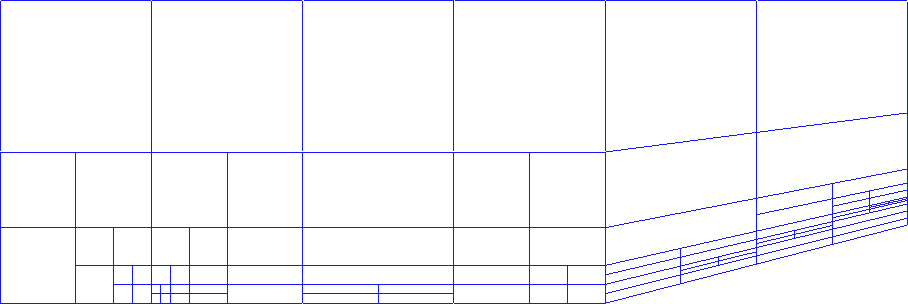
\includegraphics[width = 2.9in]{rampMesh6.png}}
\subfigure[12 refinements]{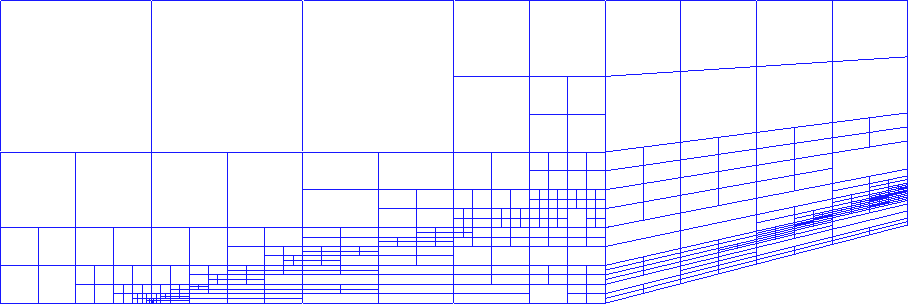
\includegraphics[width = 2.9in]{rampMesh12.png}}
\subfigure[18 refinements]{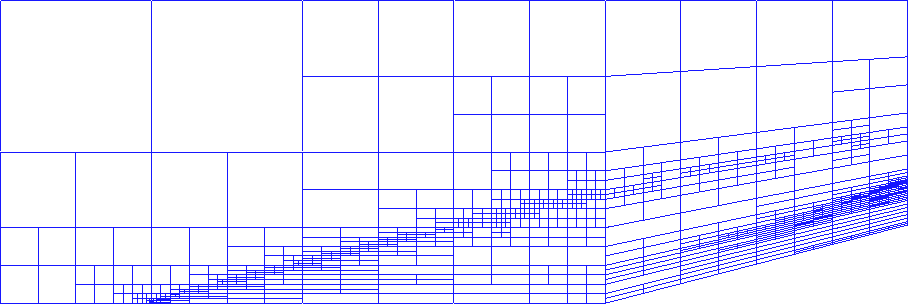
\includegraphics[width = 2.9in]{rampMesh18.png}}
\caption{Sequence of adaptive meshes for ${\rm Ma} = 6$ and $\Reyn = 10000$.}
\label{fig:holdenMa6Meshes}
\end{figure}

We can examine the sequence of adaptive meshes generated by the DPG method.  Figure~\ref{fig:holdenMa6Meshes} shows the initial mesh, as well as the 6th, 12th, and 18th subsequent refinements generated automatically by the DPG method.  Unlike the previous sequence of meshes generated by the flat plate example, refinements tend to be placed most heavily near the shock at the outflow ramp.  By the 18th refinement, the adaptive mesh looks qualitatively very similar to the final mesh of 24 refinements, and further refinements focus on the resolution of the shocks originating at the plate edge and at the ramp outflow.  

\begin{figure}
\centering
\subfigure[$\rho$ rescaled]{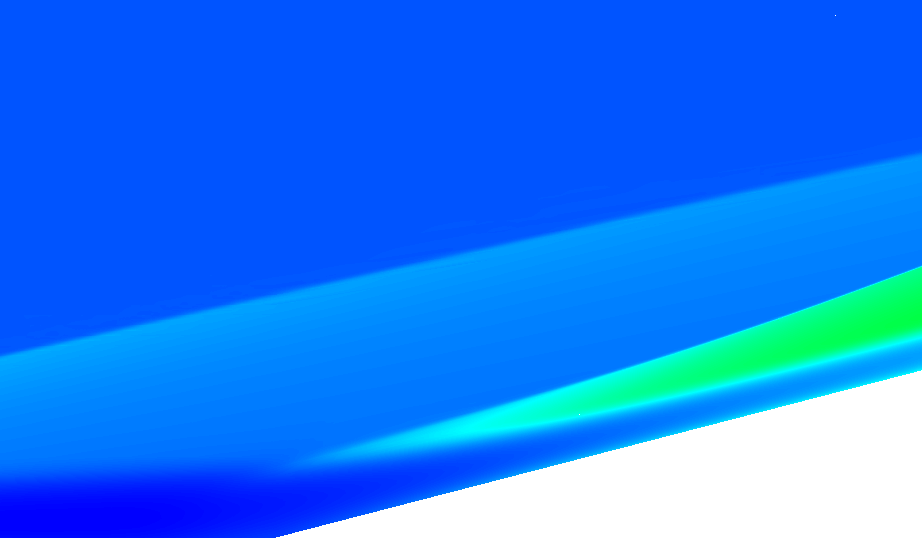
\includegraphics[width = 2.9in]{rhoRescaledshockMa6Ramp.png}}
\subfigure[$T$]{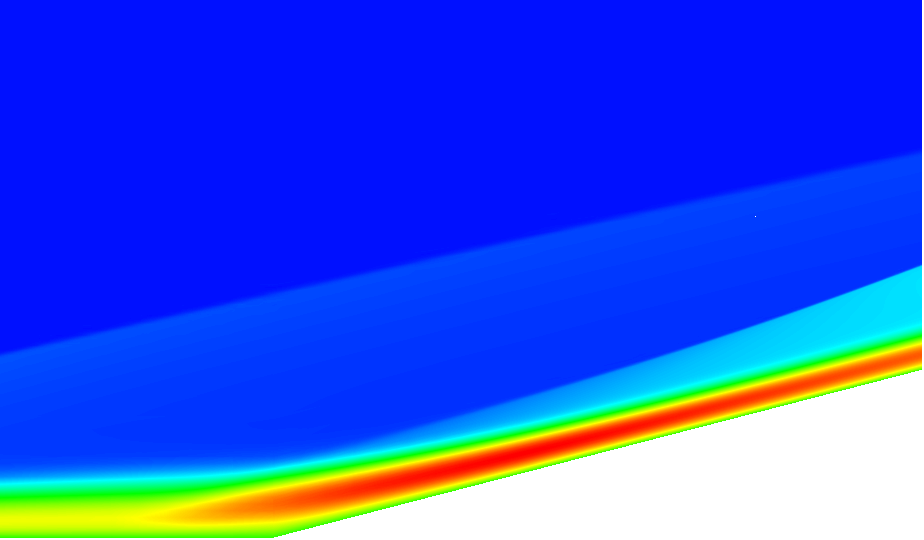
\includegraphics[width = 2.9in]{TshockMa6Ramp.png}}
\subfigure[Mesh]{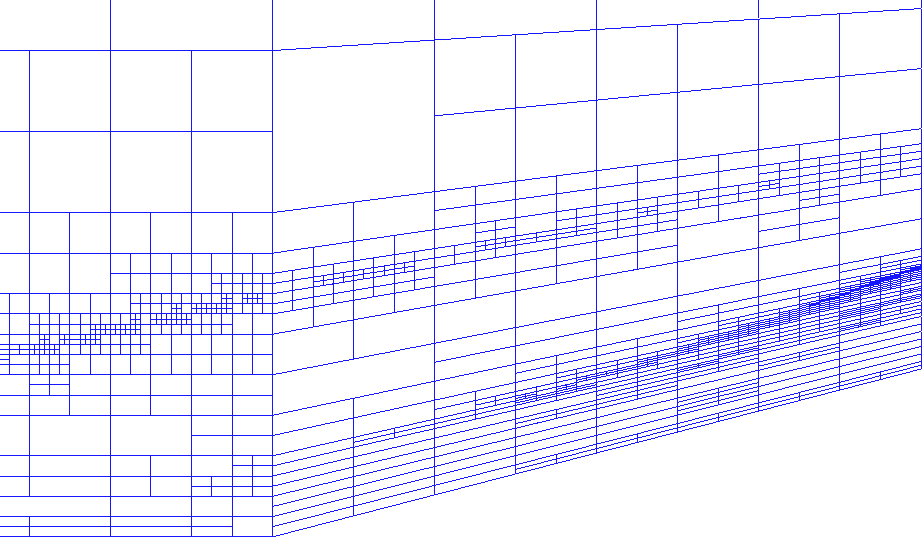
\includegraphics[width = 4in]{shockMeshMa6Ramp.png}}
\caption{Zoom of solutions and adaptive mesh around shock. }
\label{fig:holdenMa6Zoom}
\end{figure}

Figure~\ref{fig:holdenMa6Zoom} shows a zoom of the second stronger shock that develops near the ramp outflow.  Refinements are placed very heavily near the shock, which we expect due to the fact that a shock forms a stronger gradient than a boundary layer.  We note that our residual-driven adaptivity scheme places mesh refinements in a very precise manner; refinements on ramp boundary are placed slightly more heavily upstream than downstream.  We believe this is due to the fact that solution gradients are slightly higher in $\rho$ at the upstream section of the ramp.  

\begin{figure}
\centering
\subfigure[$\rho$ rescaled]{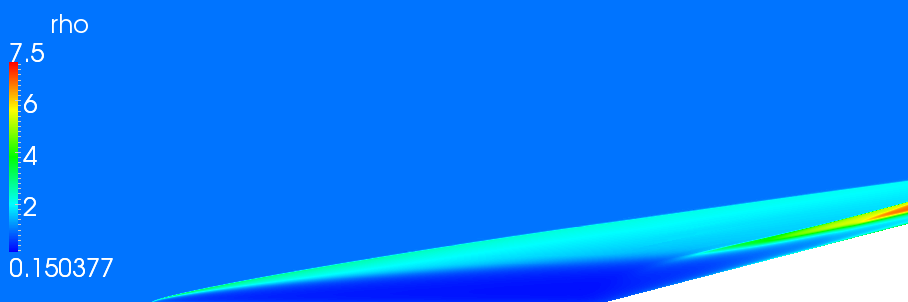
\includegraphics[width = 2.9in]{rhoRescaledMa11Ramp.png}}
\subfigure[$u_1$]{\includegraphics[width = 2.9in]{u1Ma11Ramp.png}}
\subfigure[$u_2$]{\includegraphics[width = 2.9in]{u2Ma11Ramp.png}}
\subfigure[$T$]{\includegraphics[width = 2.9in]{TMa11Ramp.png}}
\subfigure[Mesh]{\includegraphics[width = 5.5in]{meshMa11Ramp.png}}
\caption{Solutions and adaptive mesh for ${\rm Ma} = 11.68$ and $\Reyn = 16442.4$.}
\label{fig:holdenMa11}
\end{figure}

The second set of conditions under which we solve are under Mach 11.68 flow and Reynolds number of 16,4	42.4, or 55,800 if measured with respect to original plate length, with the wall temperature set to $T_{w} = 4.6T_{\infty}$.  24 automatic mesh refinements are performed under an energy threshold of $.5$, resulting in a final mesh of 2385 elements.  

Figure~\ref{fig:holdenMa11} shows the resulting solution and final adaptive mesh.  The increased Mach number changes again the angle of the weak shock resulting from the change in boundary conditions at the plate edge.  Compared to the previous case of Mach 6 flow, where only 18 refinements steps were performed, 24 refinements were performed for the Mach 11.68 case, leading to a more highly resolved solution, especially near the plate tip.  Due to a large maximum value of $\rho_{\max} = 50.1805$ at the plate tip, the resulting solution for $\rho$ is scaled to better show qualitative features of the flow.  

%We note that, under a higher Mach number, the placement of adaptive mesh refinements appears to improve.  The element size adjacent to the plate tip for the Mach $6$ case is $h = O\LRp{10^{-4}}$, while the size of elements adjacent to the plate tip in the Mach 11 case is $h = O\LRp{10^{-5}}$.  For the Mach $6$ and Reynolds $10,000$ case of the ramp problem, several extraneous refinements were placed slightly upstream of the plate tip, corresponding to the location of large gradients in the Newton solution update.  More study is necessary to determine the reasons for the difference in behavior of the automatic adaptivity algorithm.
%
%\begin{figure}[!h]
%\centering
%%\subfigure[$\rho$]{\includegraphics[width = 2.9in]{rhoshock.png}}
%%\subfigure[$T$]{\includegraphics[width = 2.9in]{Tshock.png}}
%\subfigure[Mach 6]{\includegraphics[width = 2.75in]{plateMesh.png}}
%\subfigure[Mach 11]{\includegraphics[width = 2.75in]{plateMesh.png}}
%\caption{Zoom of solutions and adaptive mesh around the plate tip.}
%\label{fig:plateComparison}
%\end{figure}

\begin{figure}
\centering
\subfigure[$\rho$ rescaled]{\includegraphics[width = 2.9in]{rhoshockMa11Ramp.png}}
\subfigure[$T$]{\includegraphics[width = 2.9in]{TshockMa11Ramp.png}}
\subfigure[Mesh]{\includegraphics[width = 4in]{shockMeshMa11Ramp.png}}
\caption{Zoom of solutions and adaptive mesh around shock. }
\label{fig:holdenMa11Zoom}
\end{figure}

Compared to the Mach 6 case, where 18 refinements were performed, the resolution of the mesh near the shock at the ramp outflow for Mach 11.68 flow and 18 refinements is qualitatively similar.  Further refinement steps increase resolution of the mesh near the shock, as shown in Figure~\ref{fig:holdenMa11Zoom}.  

Finally, we plot the normal heat flux over the plate and ramp for both Holden problems in Figure~\ref{fig:heatFlux}.  The normal heat flux over the flat plate is indicated by the blue line, while the dotted brown line indicates the heat flux over the ramp, and both are plotted against the x-coordinate along the plate/ramp boundary.  The normal heat flux is given by the normal trace of the conserved quantity in the energy equation
\[
\widehat{f}_{4,n} = (\rho e+p)u_n - \boldsymbol n\cdot \boldsymbol \sigma\cdot \boldsymbol u + q_n.
\]
Recognizing that $u_1 = u_2 = 0$ reduces the above to $\widehat{f}_{4,n} = q_n$.  

The heat flux develops a strong singularity at the point $(-.5,0)$, where the boundary condition changes from a Neumann/stress boundary condition to a Dirichlet/no-slip boundary condition.\footnote{Figure~\ref{fig:heatFlux} cuts off this singularity in order to show the qualitative behavior of $q_n$ over the remainder of the boundary.  The maximum visualized values in the singular portion of $q_n$ are .35 for Mach 6 flow and 1.268 for Mach 11.68 flow.}  It can be shown that the Laplace equation develops a singularity in stress at under any such change in boundary conditions, and the same phenomena is observed for a similar setup under convection-diffusion \cite{localConservationDPG}.  

\begin{figure}
\centering
\subfigure[Mach 6, Reynolds 10,000]{\includegraphics[width=2.9in]{heatFluxMa6Ramp.png}}
\subfigure[Mach 11.68, Reynolds 16,442.4]{\includegraphics[width=2.9in]{heatFluxMa11Ramp.png}}
\caption{Normal heat flux $q_n$ over plate and ramp for the Holden problem.  The blue line indicates $q_n$ over the flat plate, while the brown line indicates $q_n$ over the ramp. }
\label{fig:heatFlux}
\end{figure}

\subsection{Higher Reynolds numbers}
\seclab{sec:oscillations}
For higher Reynolds number, the pseudo-timestepping, we have encountered difficulties which have made it difficult to converge to a steady-state solution, even under the addition of an effective CFL number and line search to enforce positivity of density $\rho$ and temperature $T$.  However, we believe these difficulties to be related to the nature of the equations, rather than the robustness of the method.  We illustrate this with a simple example.  

Let us consider the 1D steady state viscous Burgers' equation on $[-\infty,\infty]$
\[
u\pd{u}{x} - \epsilon \pdd{u}{x} = 0.
\]
The exact solution to this equation under boundary conditions
\begin{align*}
u(-\infty) &= 1\\
u(\infty) &= -1
\end{align*}
can be easily derived (see \cite{Barter} for a simple derivation), and the solution and its first two derivatives are
\[
u(x) = \frac{1-e^{\frac{x}{\epsilon}}}{1+e^\frac{x}{\epsilon}}, \qquad u'(x) = \frac{-2e^{\frac{x}{\epsilon}}}{\LRp{1+e^{\frac{x}{\epsilon}}}^2\epsilon}, \qquad u''(x) = \frac{-2e^{\frac{x}{\epsilon}}\LRp{e^{\frac{x}{\epsilon}}-1}}{\LRp{1+e^{\frac{x}{\epsilon}}}^3\epsilon^2}
\]
\begin{figure}
\centering
\subfigure[$u(x)$]{\includegraphics[width = 1.8in]{u.pdf}}
\subfigure[$u'(x)$]{\includegraphics[width = 1.8in]{du.pdf}}
\subfigure[$u''(x)$]{\includegraphics[width = 1.8in]{ddu.pdf}}
\caption{$u(x)$ and its derivative and second derivative for $\epsilon = .01$.}
\label{fig:burgersSoln100}
\end{figure} 
Figure~\ref{fig:burgersSoln100} shows each of these functions for $\epsilon = .01$.  From the form of $u'(x)$ and $u''(x)$, we know these oscillations will grow rapidly as $\epsilon$ decreases.  Consider now the linearized Burgers' equation
\[
\pd{u\Delta u}{x} - \epsilon \pdd{\Delta u}{x} = - r(x)
\]
where $r(x) = u\pd{u}{x} - \epsilon \pdd{u}{x}$ is the strong form of the nonlinear residual.  Recall that for a pure Newton iteration, $u(x)$ is assumed to be known, and the linearized problem is driven by the residual.  The solution $u(x)$ is updated $u \coloneqq u + \Delta u$, and is repeated until $\Delta u$ and $r(x)$ are both approximately zero.

Let $u_\epsilon(x)$ be the exact solution for a particular viscosity $\epsilon$, and consider the setting of $u(x) = u_{\alpha \epsilon}(x)$, with $\alpha > 1$.  In other words, the initial guess for the Newton iteration is taken to be the exact solution for the viscous Burgers' equation under a larger viscosity (a less sharp shock), a method known as continuation (specifically, continuation in viscosity $\epsilon$).\footnote{We note that continuation in Reynolds number was attempted for the Navier-Stokes equations; however, the presence of large oscillations in the Newton update on highly adapted meshes caused the line search to return a near-zero step length, which stalled the nonlinear iteration prior to convergence to a steady state solution.}

\begin{figure}
\centering
\subfigure[$\epsilon = .01$]{\includegraphics[width = 2.5in]{residual100.pdf}}
\subfigure[$\epsilon = .001$]{\includegraphics[width = 2.5in]{residual1000.pdf}}
\caption{Residual for Burgers' equation with viscosity $\epsilon$ under the exact solution for ${2\epsilon}$.}
\label{fig:burgersResidual}
\end{figure} 

We plot $r(x)$ for $u(x) = u_{2\epsilon}(x)$ in Figure~\ref{fig:burgersResidual}.  While the form of the exact linearized solution $\Delta u$ is unknown, we see that the forcing term in the above equation develops oscillations that grow in magnitude and decrease in support as $\epsilon$ decreases.  We have observed similar behaviors for discretized solutions to the Burgers' and Navier Stokes equations -- the discrete linearized solution will develop gradients as well, though their magnitude will be limited by the resolution of the mesh.  However, additional refinements near shocks will introduce additional oscillations, which are subsequently damped by additional Newton iterations.  

In other words, not all oscillations are related to the method of discretization -- the exact linearized solution itself contains large oscillations, which are picked up more and more strongly in a discrete scheme as the mesh resolution approaches the viscous length scale $\epsilon$ (see \cite{DPGspacetime, DPGNS_1d} for additional numerical examples).  We note that these large oscillations are not an issue for the viscous Burgers' equation, as there is no positivity constraint on $u$.  However, as noted previously, the convergence of the nonlinear iteration for the compressible Navier-Stokes equations can stall or even diverge for sufficiently negative values of $\rho$ and $T$, which happens easily in the presence of large oscillations.  When a line search is implemented to enforce a strictly positive solution, the nonlinear iteration can stall, and numerical experiments have generated cases in which the line search length goes to zero, returning an under-converged solution.  

There are several approaches to controlling the magnitude of oscillations in the linearized solution -- a simple option is decreasing the size of the timestep; however, doing so can cause the number of iterations required for convergence to greatly increase.  The application of artificial diffusion near sharp gradients is another way in which to control such oscillations; however, this results in a modified set of equations, and, though solutions with contemporary artificial viscosity methods can produce solutions with expected qualitative features, there is a wide range of choices for artificial diffusion, and it was not clear in the scope of this paper which artificial viscosity method would be quantifiably superior, or most suitable for use with the DPG method.  

